% mnras_template.tex
%
% LaTeX template for creating an MNRAS paper
%
% v3.0 released 14 May 2015
% (version numbers match those of mnras.cls)
%
% Copyright (C) Royal Astronomical Society 2015
% Authors:
% Keith T. Smith (Royal Astronomical Society)

% Change log
%
% v3.0 May 2015
%    Renamed to match the new package name
%    Version number matches mnras.cls
%    A few minor tweaks to wording
% v1.0 September 2013
%    Beta testing only - never publicly released
%    First version: a simple (ish) template for creating an MNRAS paper

%%%%%%%%%%%%%%%%%%%%%%%%%%%%%%%%%%%%%%%%%%%%%%%%%%
% Basic setup. Most papers should leave these options alone.
\documentclass[a4paper,fleqn,usenatbib]{mnras}

% MNRAS is set in Times font. If you don't have this installed (most LaTeX
% installations will be fine) or prefer the old Computer Modern fonts, comment
% out the following line
%\usepackage{newtxtext,newtxmath}
% Depending on your LaTeX fonts installation, you might get better results with one of these:
%\usepackage{mathptmx}
%\usepackage{txfonts}

% Use vector fonts, so it zooms properly in on-screen viewing software
% Don't change these lines unless you know what you are doing
\usepackage[T1]{fontenc}
\usepackage{ae,aecompl}


%%%%% AUTHORS - PLACE YOUR OWN PACKAGES HERE %%%%%

% Only include extra packages if you really need them. Common packages are:
\usepackage{graphicx}	% Including figure files
\usepackage{amsmath}	% Advanced maths commands
\usepackage{amssymb}	% Extra maths symbols

%%%%%%%%%%%%%%%%%%%%%%%%%%%%%%%%%%%%%%%%%%%%%%%%%%

%%%%% AUTHORS - PLACE YOUR OWN COMMANDS HERE %%%%%

% Please keep new commands to a minimum, and use \newcommand not \def to avoid
% overwriting existing commands. Example:
%\newcommand{\pcm}{\,cm$^{-2}$}	% per cm-squared

%%%%%%%%%%%%%%%%%%%%%%%%%%%%%%%%%%%%%%%%%%%%%%%%%%

%%%%%%%%%%%%%%%%%%% TITLE PAGE %%%%%%%%%%%%%%%%%%%

% Title of the paper, and the short title which is used in the headers.
% Keep the title short and informative.
\title[Predicting extragalactic distance errors]{Predicting extragalactic distance errors using Bayesian inference in multi-measurement catalogs}

% The list of authors, and the short list which is used in the headers.
% If you need two or more lines of authors, add an extra line using \newauthor
\author[G. Chaparro-Molano et al.]{Germ\'an Chaparro-Molano,$^{1}$\thanks{E-mail: gchaparrom@ecci.edu.co}
Juan Carlos Cuervo,$^{2}$
Oscar Alberto Restrepo Gait\'an$^{1,3}$ \newauthor
Sergio Torres Arzay\'{u}s$^{4}$
\\
% List of institutions
$^{1}$Vicerrector\'ia de Investigaci\'on, Universidad ECCI, 111311 Bogot\'a, Colombia\\
$^{2}$Department, Institution, Street Address, City Postal Code, Country\\
$^{3}$Radio Astronomy Instrumentation Group, Universidad de Chile, Santiago de Chile, Chile\\
$^{4}$Centro Internacional de F\'isica, Bogot\'a, Colombia
}

% These dates will be filled out by the publisher
\date{Accepted XXX. Received YYY; in original form ZZZ}

% Enter the current year, for the copyright statements etc.
\pubyear{2018}

% Don't change these lines
\begin{document}
\label{firstpage}
\pagerange{\pageref{firstpage}--\pageref{lastpage}}
\maketitle

% Abstract of the paper
\begin{abstract}
This is a simple template for authors to write new MNRAS papers.
The abstract should briefly describe the aims, methods, and main results of the paper.
It should be a single paragraph not more than 250 words (200 words for Letters).
No references should appear in the abstract.
\end{abstract}

% Select between one and six entries from the list of approved keywords.
% Don't make up new ones.
\begin{keywords}
methods: data analysis -- methods: statistical -- galaxies: distances -- galaxies: statistics -- catalogues -- astronomical data bases: miscellaneous
\end{keywords}

%%%%%%%%%%%%%%%%%%%%%%%%%%%%%%%%%%%%%%%%%%%%%%%%%%

%%%%%%%%%%%%%%%%% BODY OF PAPER %%%%%%%%%%%%%%%%%%

\section{Introduction}


Understanding the uncertainties in redshift-independent extragalactic distance measurements is absolutely necessary before reporting statistically sound conclusions regarding the structure of the local universe \citep{void,locunivcf,nongauss,6df,localunipv,said,gg3500}, large scale structure \citep{anishub,gallargescale,morphanis,tecciencia,bayesh}, and events like transient gravitational wave detections \citep{gwgallist}. Hubble constant estimations have been using increasingly sophisticated statistical tools for primary distance determination methods, such as SNIa \citep{ridsn,unity,hubsn2018}, Cepheids \citet{hubngc} or both \citep{riess}. Although most estimates of the Hubble constant use Cepheid calibration for calibrating secondary methods \citep{hubunc,huborig,hub2010}, \citet{noceph} have explored changes in Hubble constant estimation using the Tully-Fisher relation (TF) relation without Cepheid calibration. Secondary methods for extragalactic distance determination like the TF relation, or the Fundamental Plane (FP) have recently become more precise thanks to increasing volumes of data from surveys like 6dF \citep{6df}  and  2MASS \citep{2mass,tf07dist} together with Spitzer data \citep{sorce}, along with improved statistical methods \citep{precisetf}. \\

As of 2018, three multi-measurement catalogs including a substantial amount of redshift-independent extragalactic distance measurements have been released: HyperLEDA \citep{hyperleda}, NED-D \citep{ned07,ned}, and Cosmicflows-3 \citep{cosmicflows}. HyperLEDA includes a homogenized catalog for extragalactic distances in the nearby universe, with 12866 distance measurements for 518 galaxies to date. NED-D is the NASA/IPAC Extragalactic Distance catalog of Redshift-Independent Distances, which compiles 319690 distance measurements for 182170 galaxies, for which  $\sim1800$ galaxies ($\sim1$\%) have more than 13 distance measurements, and $~180$ galaxies ($\sim0.1$\%) have distance measurements using more than 6 different methods. Cosmicflows-3 is the most up-to-date catalog, which reports distance measurements for 10616 galaxies for up to four distance determination methods, and calibrated with supernova luminosities. However, unlike HyperLEDA or NED-D, Cosmicflows-3 only reports the latest distance measurement for each method. In HyperLEDA, NED-D and Cosmicflows-3 errors are reported as one standard deviation from the reported distance modulus. Treatment of errors for combining distance moduli across methods or across measurements is suggested by \citet{ned07} and \citet{cosmicflows} to be based on weighted estimates such as the uncertainty of the weighted mean, albeit with caution due to the hererogeneous origin of the compiled data. In the case of NED-D, this is complicated by the fact that many errors are not reported or are reported as zero. In fact, the TF relation method has the largest number of galaxies with non-reported distance modulus errors (818 to date). Even though extragalactic distances measured using the TF relation were originally reported to have a relative error in distance modulus of $10-20$\% \citep{tforig}, we consider that this conservative estimate can be improved upon by using a predictive model based on the distance error of galaxies that use the same distance determination method. This requires a robust estimation of the variance of extragalactic distances based on the available data.\\

For many galaxies in all three catalogs, the random error for each distance modulus measurement $\epsilon_i$ (for $i=1,...,N$, for $N$ distance measurements per galaxy) is not representative of the scatter across measurements, even when considering the same method for determining distances. In addition, distance modulus distributions for each measurement (which are assumed to be Gaussian) are transformed to log-normal distributions in metric distance space. We improve upon previous methods by robustly estimating the underlying variance across measurements and distance determination methods for the three catalogs by bootstrap sampling the posterior distribution of each extragalactic distance \citep{chaparro18}. We compare our results to other more commonly used frequentist methods, such as the weighted estimates mentioned above. We build predictive Bayesian models for the estimation of errors and evaluate them by performing posterior predictive checks using a discrepancy measure and a Bayesian ``p-value'' \citep{gelmanppd}. Furthermore, we make predictions for the 818 galaxies in the NED-D catalog whose distances were measured using the TF relation but have non-reported errors. The usefulness of posterior predictive checks on Bayesian models for inference has been discussed in \citet{gelman2003} and \citet{ppcinf}.\\

We organized this paper as follows. In Section~\ref{sec:post} we talk about the posterior distribution of distance for individual galaxies and set up methods for measuring its variance. In Section~\ref{sec:comp} we make a comparison between the proposed variance estimation methods, and in Section~\ref{sec:predbay} we propose and evaluate predictive Bayesian models for two robust methods of error estimation, and we summarize our work in the Conclusions section.

\section{Posterior distribution for extragalactic distances}
\label{sec:post} 
 
As mentioned in the Introduction, the best approach to consider the effects of random and scattering errors in catalog-wide, multi-method distance analyses is to perform a robust estimation of the variance of the posterior distribution of each extragalactic distance. The posterior distribution of the distance to a given galaxy can be obtained by drawing distance modulus bootstrap samples from $P(\mu)$, which is the unweighted mixture of normal distributions corresponding to each distance modulus measurement $\mu_i$,
\[\mu\sim\sum_i^N \mathcal{N}(\mu_i,\epsilon_i^2)\ ,\]
and then converting to metric distance,
\[D=10^{\frac{\mu}{5}+1}\ .\]
Therefore,
\[D_G\sim\sum_i^N\mathrm{lognormal}(M_i,\sigma_{M_i}^2)\ .\]
Here $M_i=\ln D_i$ and $\sigma_{M_i}=\epsilon_i\cdot\ln10$.\\

However, this method is not very efficient for a standardized treatment of errors. It is more convenient to treat each extragalactic metric distance $D_G$ as a normal random variable with a single-valued $\sigma_D$ as a measure of the uncertainty in the estimation of an extragalactic distance,
\[D_G\sim \mathcal{N}(D,\sigma_D^2)\]
For this reason we compare four methods for estimating the $D,\,\sigma_D$ pair. Two of these methods (H, M) use robust measures of the posterior distribution of each extragalactic distance, and the other two (P, Q) use measures based on propagation of errors.

\subsection{Estimating the variance of $P(D_G)$}
\label{sec:meth} 

Method H takes $D$ as the median of the posterior and $\sigma_D$ as the half-distance (H) between the 84th and 16th percentiles of the posterior. Method M takes $D$ as the median of the posterior and $\sigma_D$ as the median absolute deviation (MAD) of the posterior. Method P consists on calculating $D$ from the weighted mean distance modulus $\bar{\mu}^*$ with weights $w_i=\epsilon_i^{-2}$. $\sigma_D$ is calculated by propagation (P) of measurement errors  i.e. from the uncertainty of the weighted mean \citep{cosmicflows},
\begin{equation}
\sigma_D^P=0.461\,\bar{D}^*\,\left(\sum_i^Nw_i\right)^{-1/2} \ ,
\end{equation}
Method P does not take into account the scatter in distance measurements for single galaxies, which is why method Q calculates $D$ same as method P, but $\sigma_D$ is calculated as the sum in quadrature (Q) of the propagated uncertainty of the weighted mean and the propagated unbiased weighted sample variance $\sigma_D^*$:
\begin{equation}
\sigma_D^Q=\left[ \left(\sigma_D^P\right)^2+\Big(\sigma_D^*\Big)^2\right]^{1/2} \ .
\end{equation}
Here $\sigma^*_D$ is calculated as  \citep{wstdev},
\begin{equation}
\sigma^*_D=0.461\,\bar{D}^*\,\sqrt{\frac{N}{N-1.5}\frac{\sum_i^Nw_i(\mu_i-\bar{\mu}^*)^2}{\sum_i^Nw_i}\vphantom{\Biggl(}}\ .
\end{equation}
If the non-robust P and Q methods are representative of the variance of the posterior, they should yield similar results as the H method. Next section shows that this is not the case.

\subsection{Comparison of variance estimation methods}
\label{sec:comp} 


Even though our analysis for error estimation can be used to combine distance measurements using different methods for single galaxies, we think that due to method-intrinsic systematics it is more appropriate to separate the analysis by method. A full discussion of our error estimation method applied to multi-method measurements in the HyperLEDA, NED-D and Cosmicflows-3 is given in the appendix. A live, Binder-compatible repository for this work is located at \texttt{https://github.com/saint-germain/anisotropias}. Without loss of generality, we focus on galaxies whose distances have been measured using the Tully-Fisher method in the NED-D catalog because it is the method with the largest number of galaxies without reported measurement errors (818) in the database. From here on, when we mention distance measurements in the NED-D catalog, we will be excluding from our analysis measurements that require the target redshift to calculate the distance, as indicated in the \texttt{redshift (z)} field. \\

For galaxies with a number of TF distance measurements between 2 and 5, errors estimated with the the quadrature (Q), and median absolute deviation (M) methods show a linear trend with similar slopes (Fig.~\ref{fig:hpmlow}) that overpredict the variance with respect to the half 84th-16th percentile distance (H) method, whereas the propagation (P) method tends to underpredict the errors. Furthermore, errors estimated using the Q method show a larger dispersion around the linear trend than the H and M methods. The central limit theorem indicates that as the number of measurements increases, the behavior of the distance errors should settle toward being normally distributed around the correlation trend. Fig.~\ref{fig:comp} shows that for a small but representative sample of galaxies with more than 7 distance measurements, the center and variance of the posterior distribution of each extragalactic distance is best explained using the H method, whereas the less robust P and Q methods under-predict the variance. The M method also under-predicts the variance because it is a robust method, and thus not as sensitive to outliers as methods P and Q, as seen in the case of NGC 1558 in Fig.~\ref{fig:comp}. For the more symmetrical posterior distribution of UGC 12792, the M and Q methods predict the same center and variance. Fig.~\ref{fig:hqp} shows that the Q and P methods underpredict distance errors for galaxies with more than 5 TF distance measurements. Fig.~\ref{fig:qm} shows that method Q underpredicts distance errors with respect to the M method, which again shows a tighter linear correlation due to its robustness. The general correlation between distance and distance error (Figs.~\ref{fig:hqmlow} and \ref{fig:hqp}) means that there is a strong systematic component in the variance of $P(D_G)$, which is expected from the distance modulus to metric distance conversion. To improve visualization, only errors for galaxies with more than 5 TF distance measurements are shown in Figs.~\ref{fig:qm}, \ref{fig:ee}, \ref{fig:predl1}, and \ref{fig:predl2}.\\

\begin{figure*}
	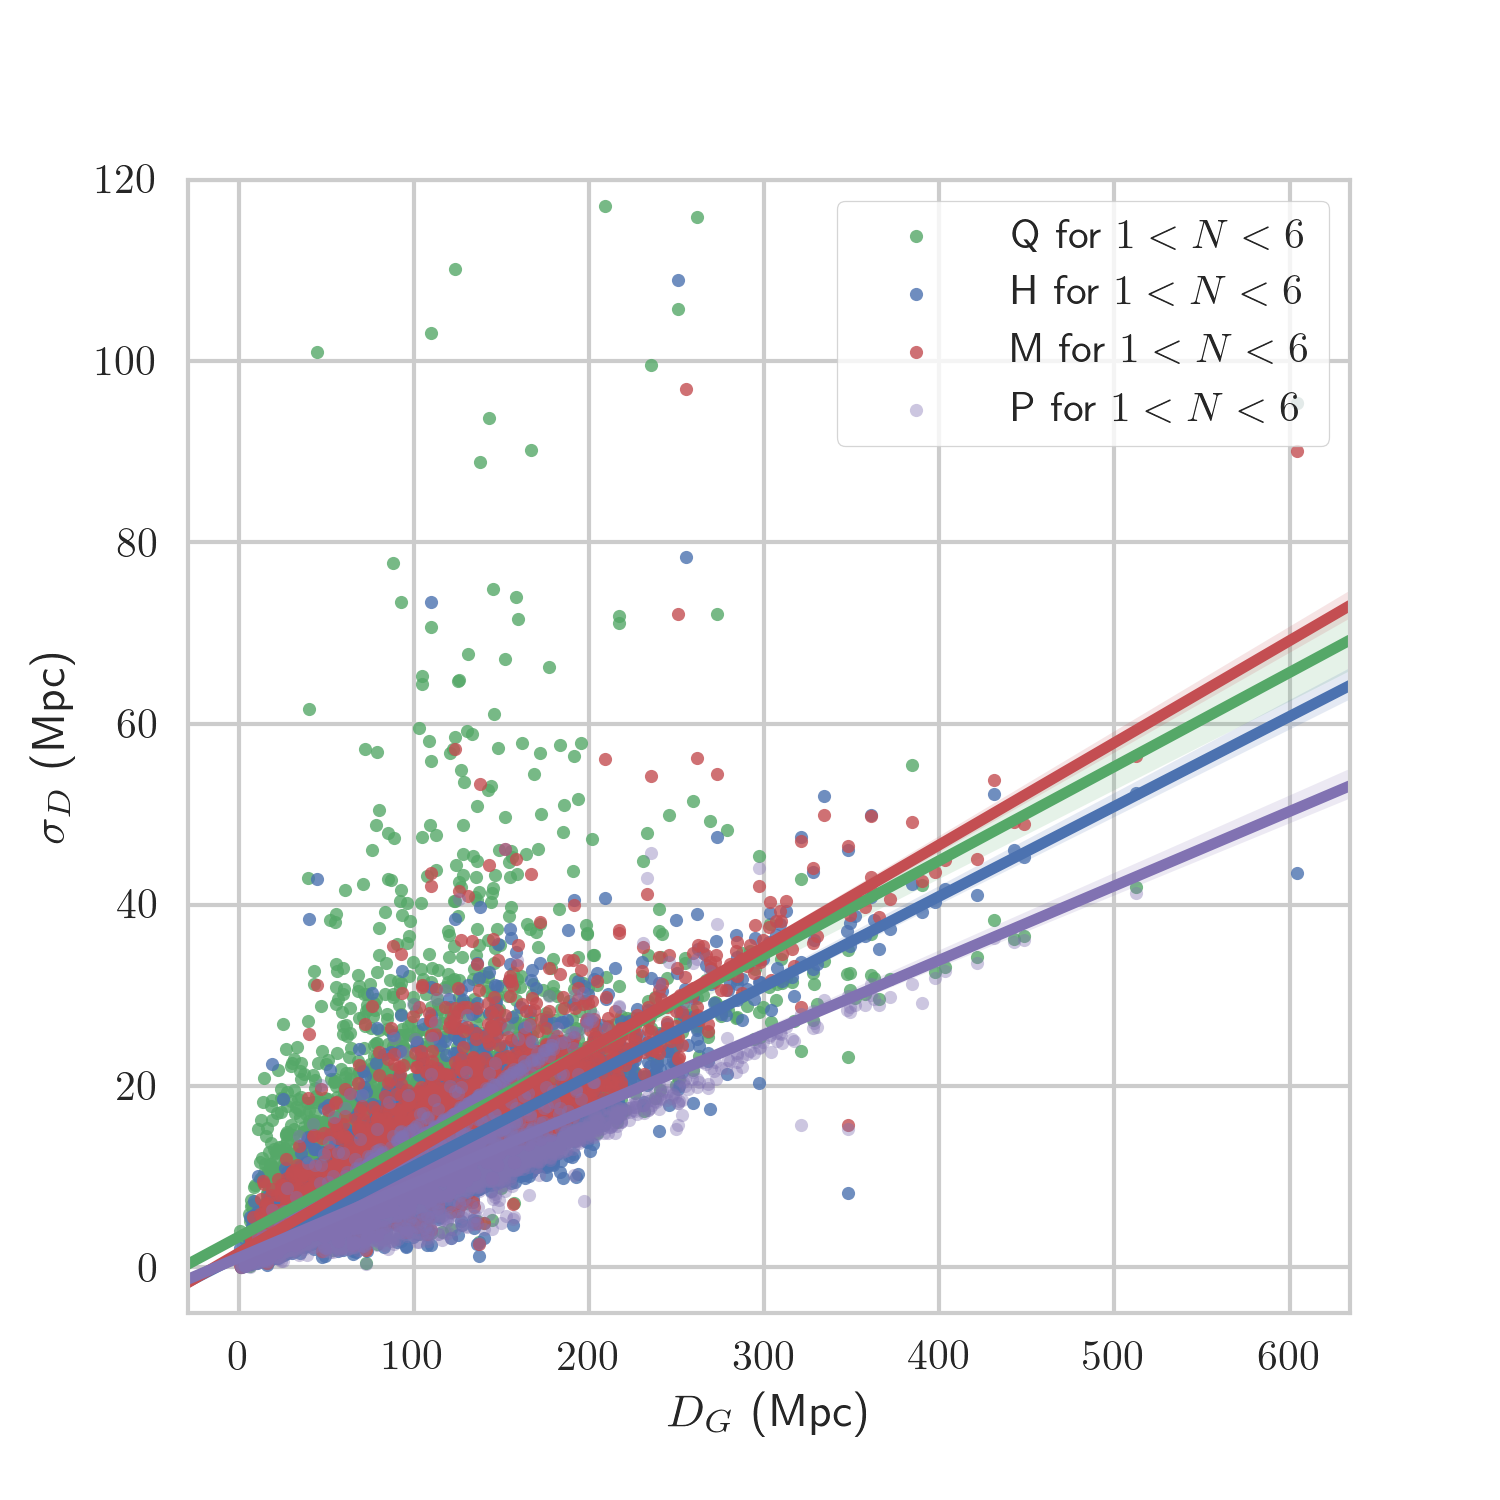
\includegraphics[scale=0.7]{hqmlow.png}
    \caption{Median extragalactic distance vs. predicted extragalactic distance errors for galaxies with a number of TF distance measurements between 2 and 5 in NED-D according to the Q, H, M, P error models (explained in the text), showing a linear regression and confidence intervals computed using the \texttt{seaborn.regplot} Python function.}
    \label{fig:hqmlow}
\end{figure*}

\begin{figure*}

	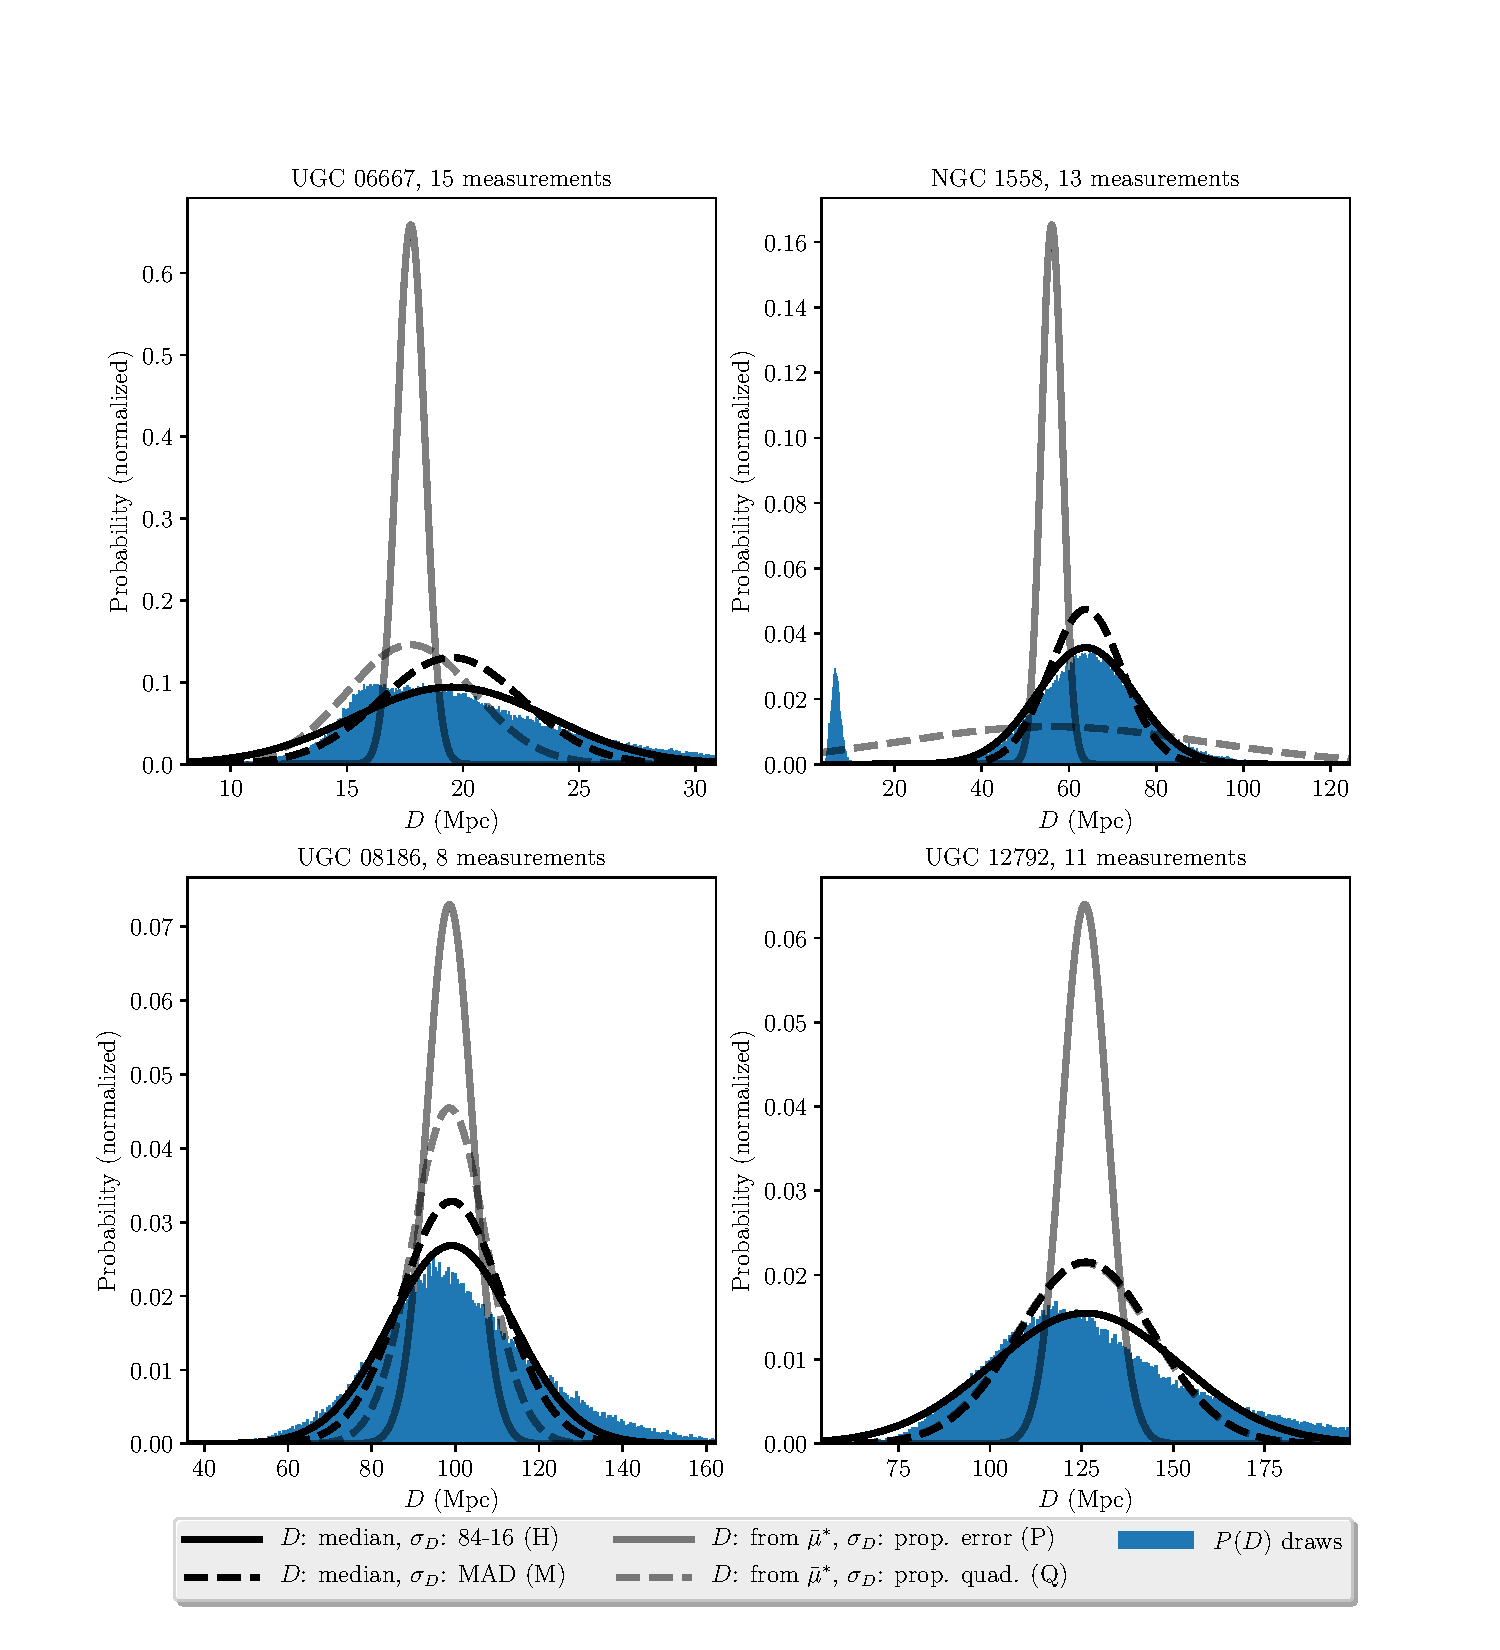
\includegraphics[scale=0.7]{comp}
    \caption{Comparison of extragalactic distance posterior distribution draws (10000 per measurement) and modeled distributions for UGC 06667, NGC 1558, UGC 08186, and UGC 12792 using the Tully-Fisher Method for distance determination in NED-D. The four methods used for approximating the posterior distribution (H, M, P, and Q) are described in the text. }
    \label{fig:comp}
\end{figure*}

\begin{figure*}

	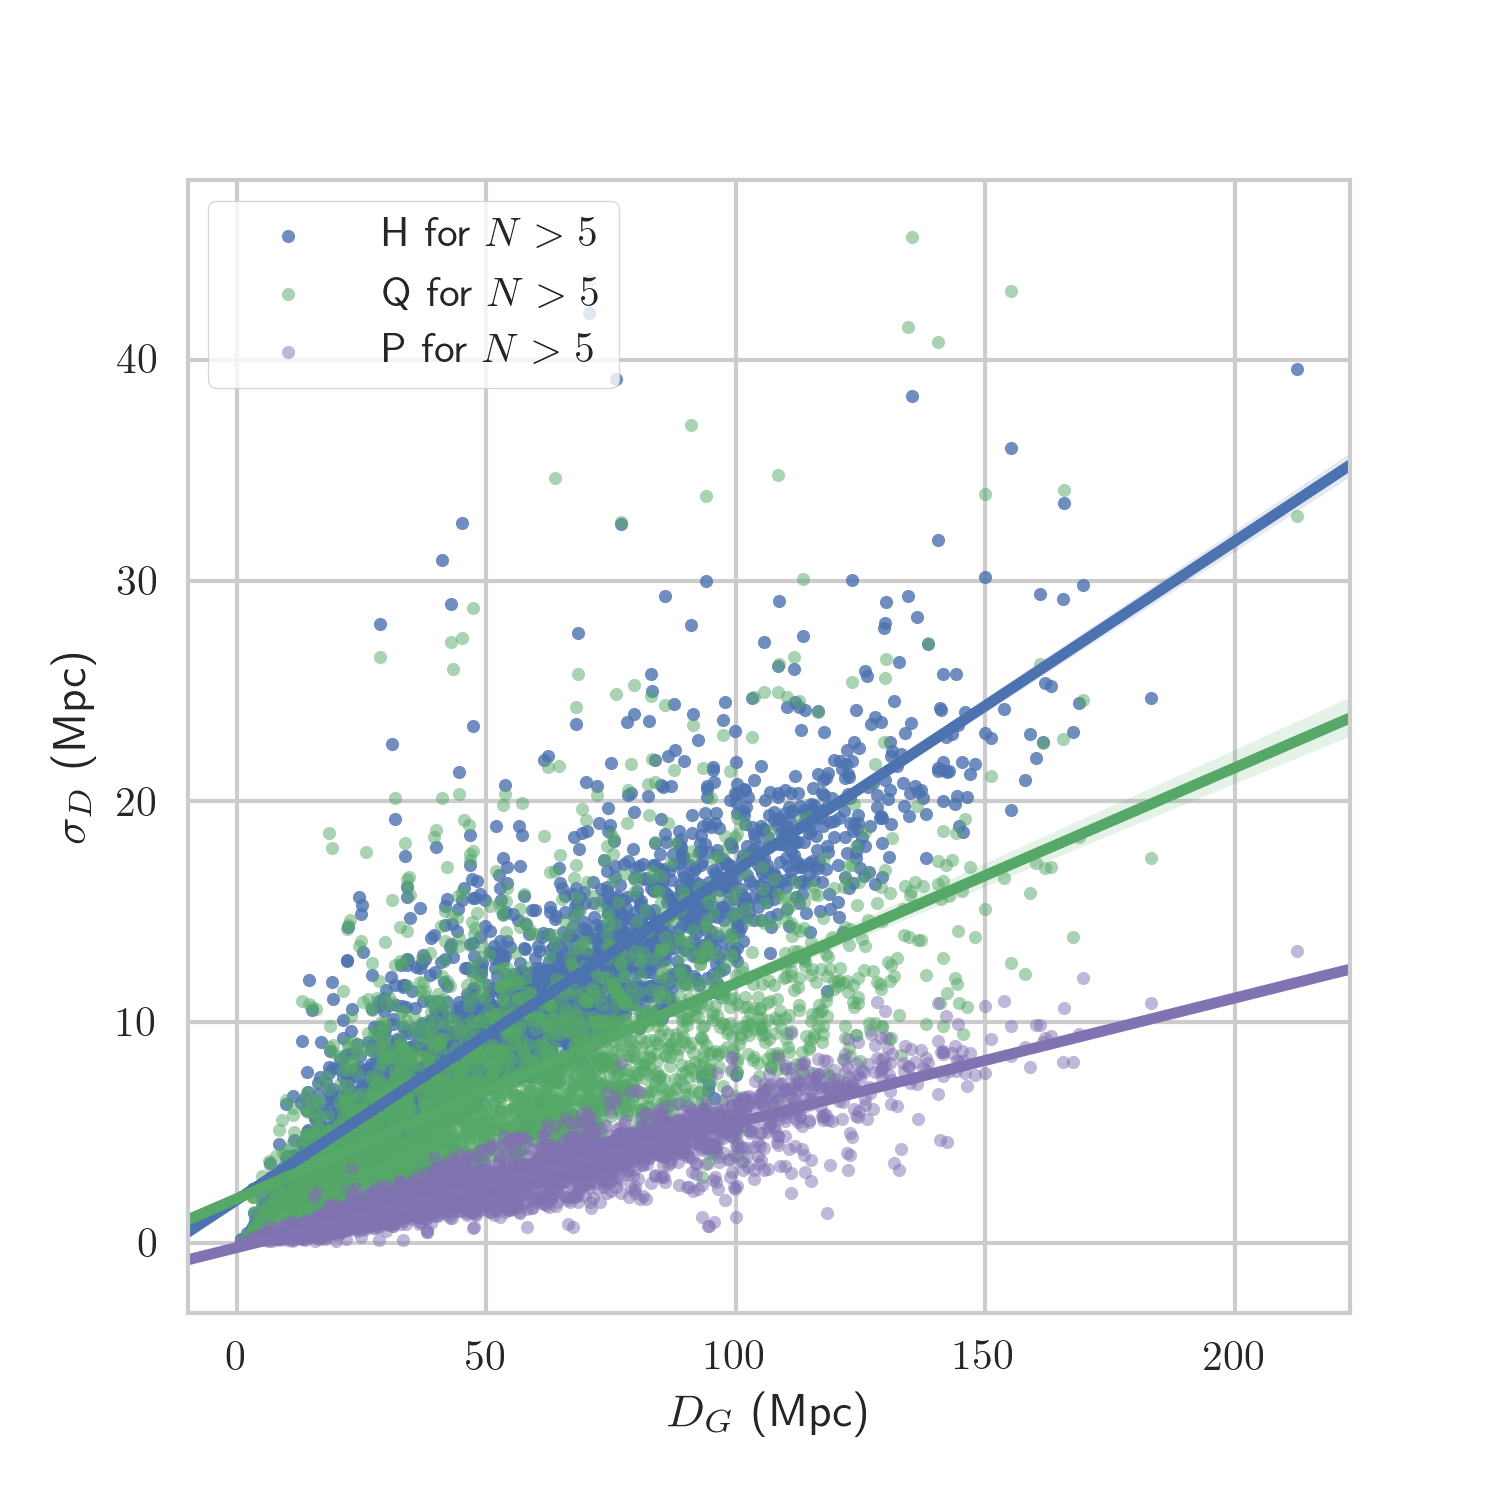
\includegraphics[scale=0.7]{hqp.png}
    \caption{Median extragalactic distance vs. predicted extragalactic distance errors for galaxies with more than 5 TF distance measurements in NED-D according to the H, Q, P error models, showing a linear regression and confidence intervals computed using the \texttt{seaborn.regplot} Python function.}
    \label{fig:hqp}
\end{figure*}

\begin{figure*}

	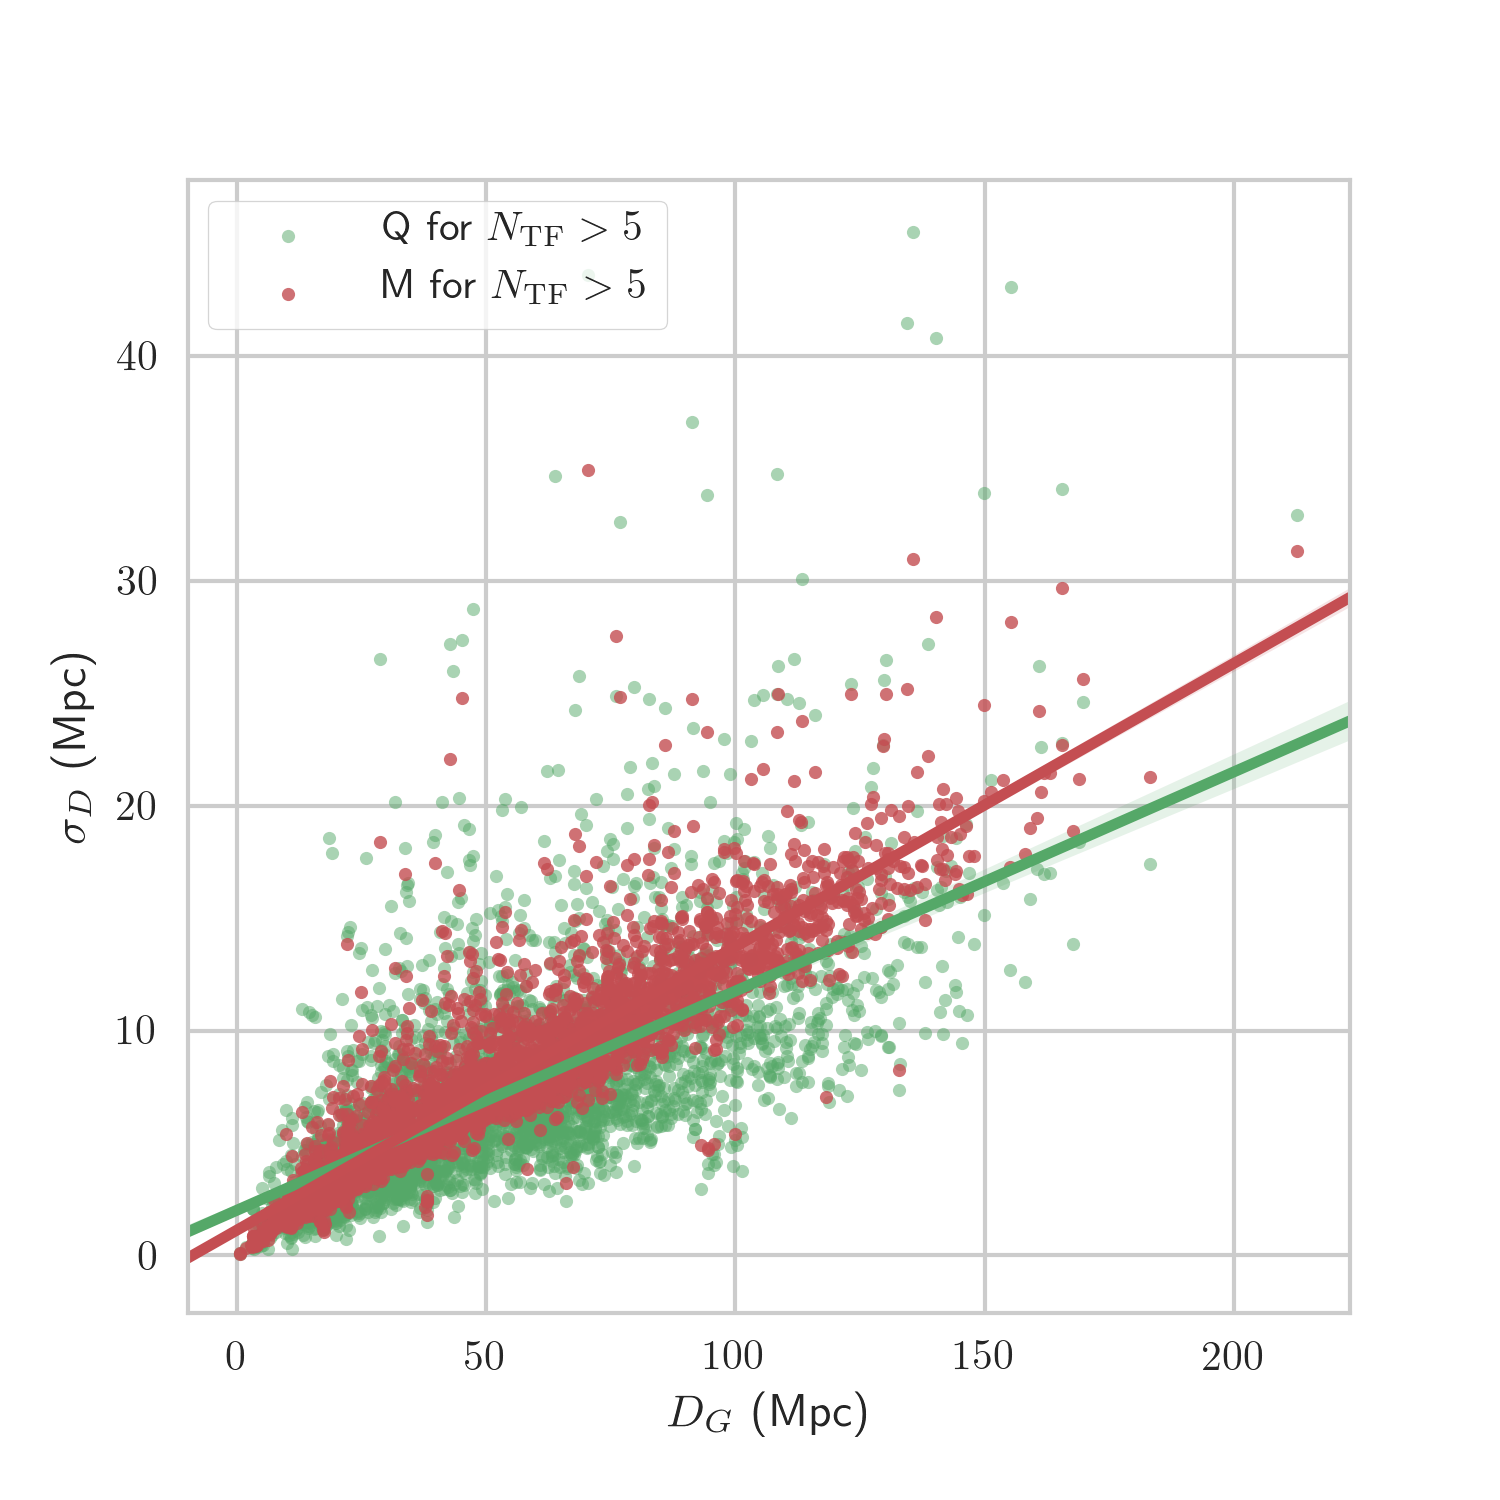
\includegraphics[scale=0.7]{qm.png}
    \caption{Median extragalactic distance vs. predicted extragalactic distance errors for galaxies with more than 5 TF distance measurements in NED-D according to the Q, M error models, showing a linear regression and confidence intervals computed using the \texttt{seaborn.regplot} Python function.}
    \label{fig:qm}
\end{figure*}

\begin{figure*}

	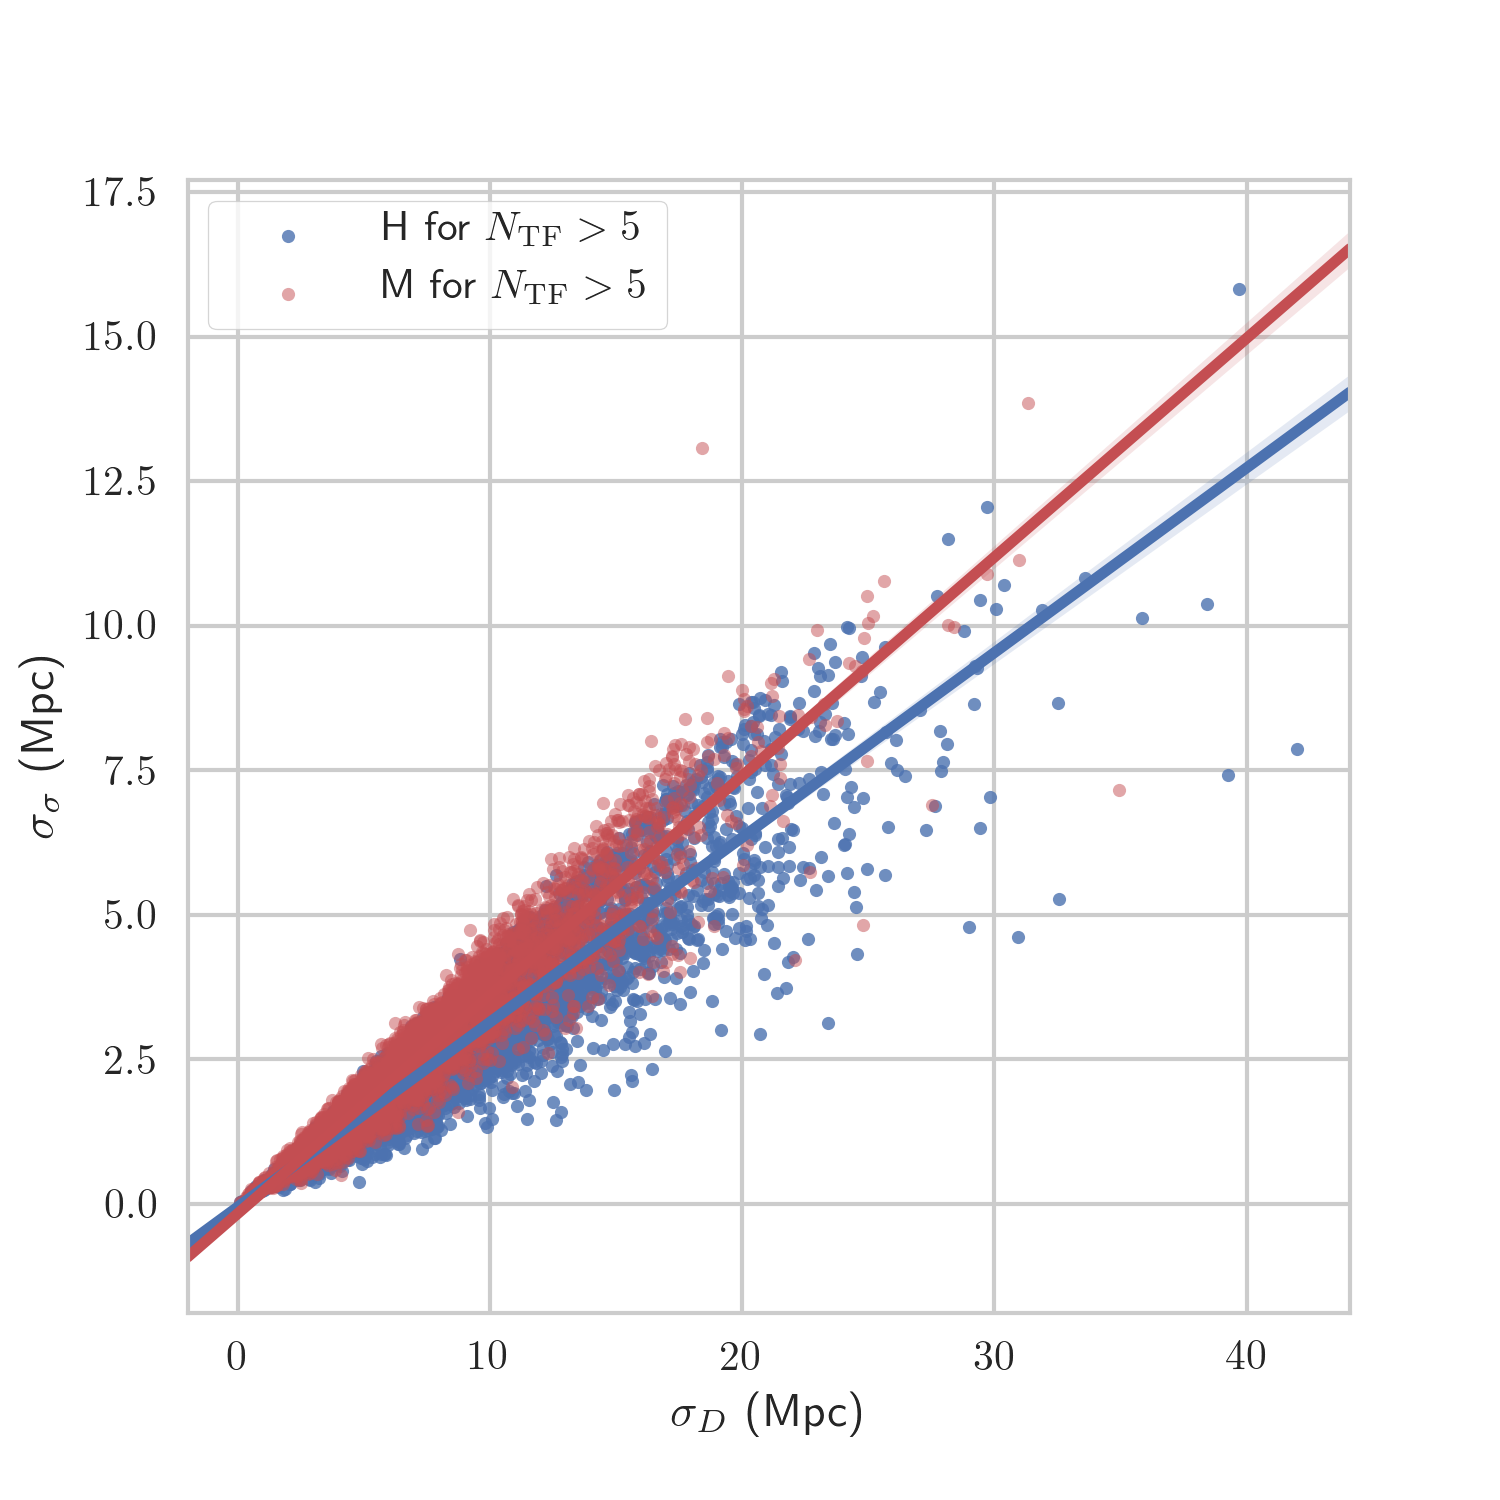
\includegraphics[scale=0.7]{ee.png}
    \caption{Predicted extragalactic distance errors vs. variance of the error as determined by the H and M methods, showing a linear regression and confidence intervals computed using the \texttt{seaborn.regplot} Python function. }
    \label{fig:ee}
\end{figure*}

Given that each $\sigma_D$ calculated using the H and M methods is obtained from many realizations from the posterior distribution of extragalactic distances, it is also possible to calculate its variance as the half-distance between the 84th and 16th percentile of bootstrap $\sigma_D$ realizations. Fig.~\ref{fig:ee} shows that the variance of the estimated error is proportional to the error for the H and M methods. This will be relevant in Section~\ref{sec:predbay} when we construct a predictive model for non-reported errors.

\section{Predictive Bayesian Models for TF missing errors}
\label{sec:predbay} 

As seen in Figs.~\ref{fig:hqp} and \ref{fig:qm}, TF distance errors estimated using the robust methods H and M grow in a roughly linear fashion with distance, but are randomly distributed around this trend line. For this reason we try out several Bayesian models in order to be able to predict missing distance errors. For this, we use the \texttt{emcee} affine invariant Markov Chain Monte Carlo (MCMC) ensemble sampler \citep{emcee}. Recently, \texttt{emcee} has been proved to be useful in obtaining probabilistic estimations for photometric redshifts \citet{photred1,photred2}. Since we want to be able to predict non-reported errors, our model selection is based on posterior predictive checks, i.e. we rely on models that can create synthetic datasets similar to the original dataset \citep{gelmanppd}. This allows us to reproduce the original variance of the error (Fig.~\ref{fig:ee}. Many Bayesian analyses often do not use posterior predictive checks, like in the work of \citet{propprob2018} and \citet{bayesh}, where they used \texttt{emcee} for posterior sampling, and using Bayesian and Akaike Information Criteria along with Bayes factors for model assessment, but without attempting to reproduce the original variance of the data. This is also the case in other Bayesian tools like Linmix  \citep{gmastro}, which is widely used in astronomy for approximating unobserved data.  \\

First we assume that for any galaxy $j$ the distance error $\sigma_{Dj}$ is a random normal variable, with variance $\sigma_{\sigma j}$ and mean $\hat{\sigma}_{Dj}$, 
\begin{equation}
P(\sigma_{Dj}|\hat{\sigma}_{Dj},\sigma_{\sigma j})=\mathcal{N}(\hat{\sigma}_{Dj},\sigma_{\sigma j}^2)\ .
	\label{eq:prob}
\end{equation}
Our likelihood function is the joint probability that each of the $\sigma_D=\{\sigma_{Dj}\}$ in the original dataset of $m$ galaxies is generated by the above probability,  
\begin{equation}
 P(\sigma_{D}|\hat{\sigma}_{D},\sigma_{\sigma})=\prod_j^mP(\sigma_{Dj}|\hat{\sigma}_{Dj},\sigma_{\sigma j})
\end{equation}
We want to test the hypothesis mentioned above that all errors and their variances $(\hat{\sigma}_D=\{\hat{\sigma}_{Dj}\},\ \sigma_\sigma=\{\sigma_{\sigma j}\})$ can be estimated from a single model depending on the extragalactic distances $D_G=\{D_{Gj}\}$ and a set of distance-independent parameters $\pmb{\theta}$. Thus the likelihood can be expressed as,
\[P(\sigma_D|D_G,\pmb{\theta})=\prod_j^mP(\sigma_{Dj}|D_{Gj},\pmb{\theta})\ .\]
Following Bayes' theorem we can compute the posterior probability up to a constant,
\begin{equation}
P(\pmb{\theta}|D_G,\sigma_D)\propto P(\pmb{\theta})P(\sigma_D|D_G,\pmb{\theta})\ .
	\label{eq:ppd}
\end{equation}
Due to the simplicity of the models used here, we will only use conservative (flat) priors. From our analysis of Fig.~\ref{fig:ee}, all our models take $\sigma_\sigma=f\hat{\sigma}_D$. This error variance scale factor $f$ is therefore one of the parameters in $\pmb{\theta}$. On the other hand, our models will differ by the proposed functional forms of $\hat{\sigma}_D(D_G,\pmb{\theta})$.\\

We obtain a computationally credible sampling of the posterior probability by removing the burn-in steps of the random walk according to the autocorrelation time. We can then create synthetic datasets by drawing a parameter sample $\pmb{\theta}_k$ from the posterior and using it to draw from the likelihood to create a new dataset, i.e. drawing new $\sigma_{Dj}$ from the probability distribution for all galaxies in the original dataset using equation~\ref{eq:prob}. We then assess the validity of the model by comparing synthetic data with the observed (i.e. original) data. This comparison is done by using a discrepancy measure $\mathcal{D}(\sigma_D|\pmb{\theta}_k)$ between data and model-derived expected values for the same data $e=\{e_j(\pmb{\theta}_k)\}$, where $\theta_k$ is drawn from the posterior distribution and $\sigma_D$ can be the observed errors or the model-generated synthetic errors. The discrepancy can be calculated using a statistic like $\chi^2$ \citep{chi2ms,otherdisc}, but here we will work with the Freeman-Tukey discrepancy since it is weight independent \citep{bishopft,brooks}, 
\[\mathcal{D}(\sigma_D|\pmb{\theta}_k)=\sum_j^m(\sqrt{\sigma_{Dj}\vphantom{e_j(\pmb{\theta}_k)}}-\sqrt{e_j(\pmb{\theta}_k)})^2\]
For each parameter draw $k$, it is possible to compare the symulated discrepancy with the observed discrepancy. If the model is representative of the data, then for many parameter draws, the symulated and observed discrepancies should be similar. We can then calculate a Bayesian ``$p$-value'' as the ratio of ``draws when the observed discrepancies are larger than the synthetic discrepancies'' to ``total draws''. If this Bayesian $p$-value is too close to 0 or to 1 we can reject the model, otherwise we cannot reject the model, as it is generating synthetic data that is similar to the original data. This is better visualized using a discrepancy plot, where for each draw $k$, a synthetic discrepancy is paired with its corresponding observed discrepancy. If the discrepancy points are roughly equally distributed about the $\mathcal{D}_\mathrm{obs}=\mathcal{D}_\mathrm{sym}$ line, then we cannot reject the model. We expect that galaxies with the largest number of measurements are sampling more completely the ``true'' distribution of the distance. Therefore we expect that if we set an increasing limit on the minimum number of measurements per galaxy on the dataset that goes in the model, the Bayesian $p$-value will improve.

\subsection{Bayesian Quadrature Model}
\label{sec:bqm} 

Our first model is based on the hypothesis that there are are distinct systematic and random contributions to the distance measurement error, both of which are normally distributed. For this reason they are added in quadrature, 
\begin{equation}
\sigma_D^2=\sigma_s^2+\sigma_r^2\ .
	\label{eq:bayq}
\end{equation}
Here $\sigma_r$ is a random (constant) error and the systematic error is modeled allowing for scale factor ($s$) and zero setting ($a$) errors, i.e.  $\sigma_s=sD+a$, as Fig.~\ref{fig:hqp} suggests.  We set our prior to be symmetrical around $\sigma_r=0$ in order to better visualize its behavior near this point, so
\begin{equation}
P(s,a,\sigma_r)=\left\{
\begin{aligned}
1,\ \ \ \ &\mathrm{if}\ \ \ 0<s<1\ \mathrm{and}\\
& \ \ \ \ \  0<a<10\ \mathrm{Mpc}\ \mathrm{and}\\
&-10<\sigma_r<10\ \mathrm{Mpc}\ \mathrm{and}\\
& \ \ \ \ \  0<f<1\\
0,\ \ \ \ &\ \mathrm{otherwise.}
\end{aligned}
\right.
	\label{eq:priorq}
\end{equation}
We now use \texttt{emcee} to sample the posterior over the parameter set $\pmb{\theta}=(s,\sigma_r,f,a)$ using 100 walkers and 20000 steps ($t_\mathrm{autocorr} \lesssim 90$ steps). According to the discrepancy plot in Fig.~\ref{fig:discq}, this model is able to replicate method H errors for the 29 galaxies with $N>25$ measurements (812 measurements in total). The corner plot showing the posterior sampling made by \texttt{emcee} is shown in Fig.~\ref{fig:cornerq}, which shows that the systematic scale factor error is $s=0.24_{-0.03}^{+0.03}$, the random error component is $\sigma_r=-0.004_{-1.296}^{+1.294}$ Mpc, the error variance scale factor is $f=0.24_{-0.03}^{+0.04}$, and the zero offset systematic error is $a=0.43_{-0.34}^{+0.56}$\ Mpc. From the large variance in the marginalized posterior distribution for $\sigma_r$ and $a$, we see that there is a significant degeneracy between those parameters. However, it should be noted that the marginalized posterior distribution of $\sigma_r$ is symmetric around zero (because of its own degeneracy), while the distribution of $a$ can only take positive values. The working distance range and overall fitting of this model is shown in Fig.~\ref{fig:drawsq}, where the method H errors corresponding to galaxies with more than 25 TF distance measurements are plotted along the expected values $e=\{e_j(\pmb{\theta}_k)\}$ for parameter sets $\pmb{\theta}_k$ drawn from the posterior probability distribution. 
\begin{figure*}
	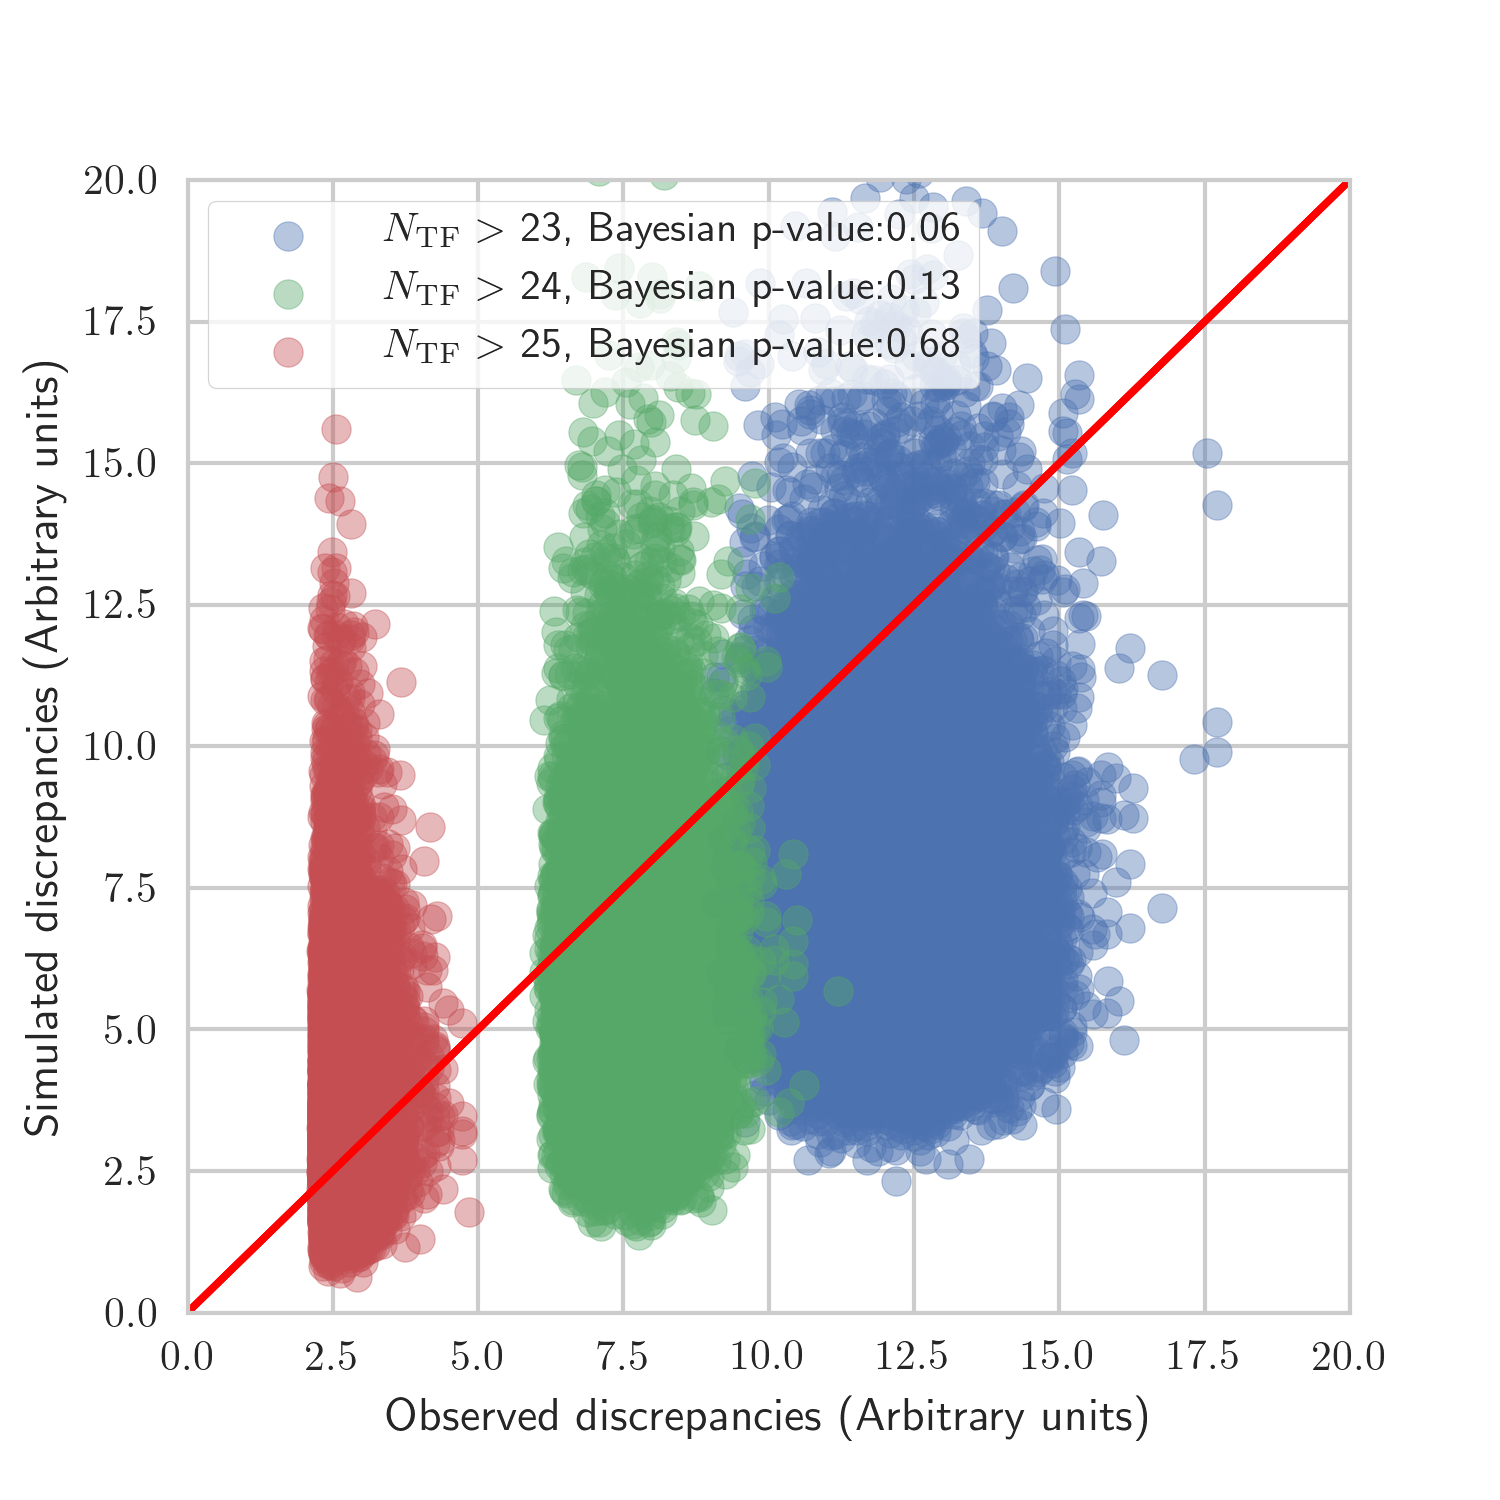
\includegraphics[scale=0.7]{discq.png}
    \caption{Discrepancy plot for the Bayesian quadrature model (equation~\ref{eq:bayq}) based on errors estimated using method H. }
    \label{fig:discq}
\end{figure*}
\begin{figure*}
	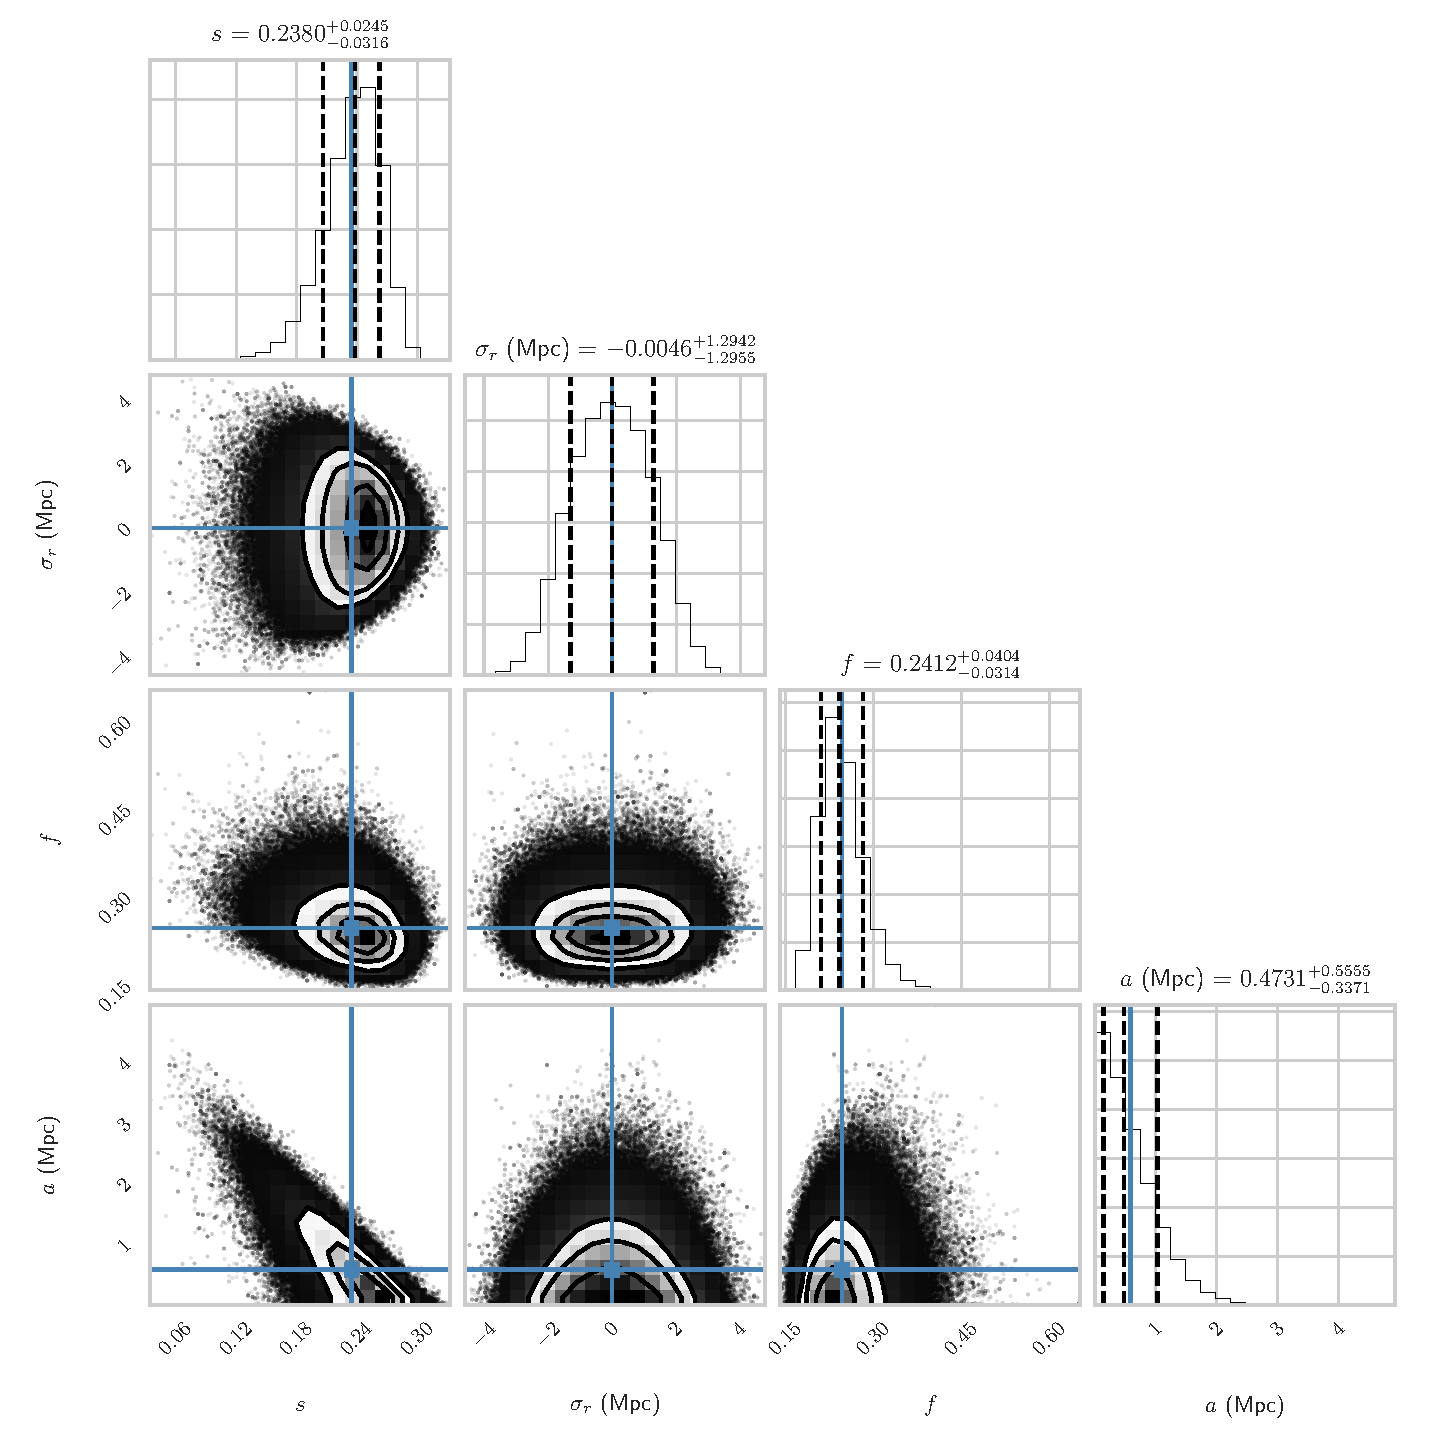
\includegraphics[scale=0.7]{cornerq}
    \caption{Corner plot showing the \texttt{emcee} sampling of the posterior probability distribution (equation \ref{eq:ppd}) for the quadrature Bayesian model parameters $\pmb{\theta}=(s,\sigma_r,f,a)$ based on errors estimated using method H for galaxies with more than 25 TF distance measurements. The dashed lines indicate the 16th, 50th, and 84th percentile of the marginalized distribution of each parameter (shown at the top of each column), and the blue solid lines indicate the mean. This plot was made using the \texttt{corner} Python module.}
    \label{fig:cornerq}
\end{figure*}
\begin{figure*}
	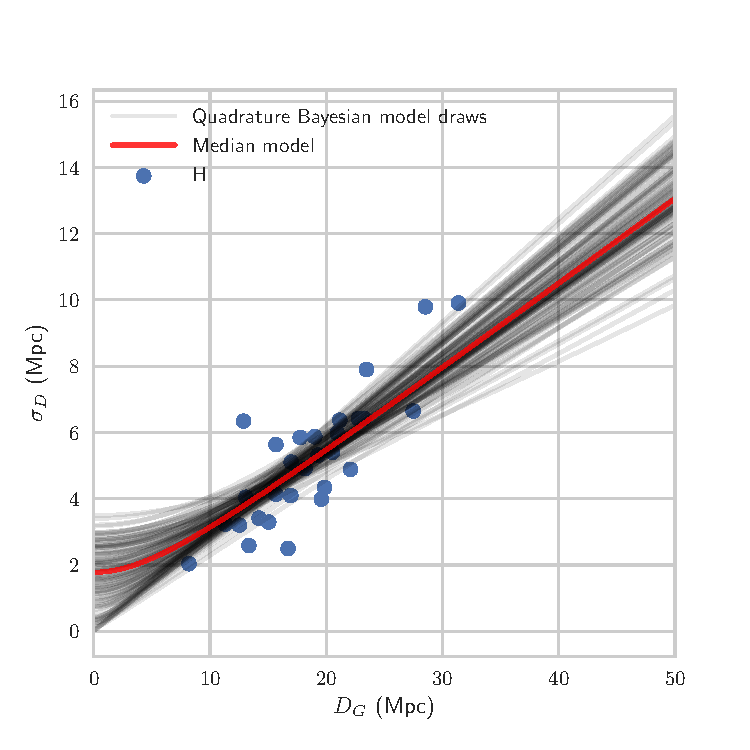
\includegraphics[scale=0.7]{drawsq}
    \caption{Projection of parameter set samples from the posterior probability distribution of the Bayesian quadrature model onto the $D_G$ vs. $\sigma_D$ scatter plot for errors estimated using method H for galaxies with more than 25 TF distance measurements.}
    \label{fig:drawsq}
\end{figure*}
Now we sample the posterior distribution for the Bayesian quadrature model with method M errors using \texttt{emcee} with 100 walkers and 20000 steps s ($t_\mathrm{autocorr} \lesssim 50$ steps). The discrepancy plot for method M errors in Fig.~\ref{fig:discq2} shows that the quadrature model also replicates method M errors, but for the 727 galaxies with more than 13 measurements (12947 measurements in total). Fig.~\ref{fig:cornerq2}, shows that $s=0.142_{-0.003}^{+0.003}$, $\sigma_r=0.004_{-0.201}^{+0.201}$ Mpc, $f=0.228_{-0.006}^{+0.007}$, and $a=0.52_{-0.06}^{+0.06}$ Mpc. The random error is so low that the model draws are almost indistinguishable from straight lines in Fig~\ref{fig:drawsq2}. Additionally, and just as for the quadrature model for H errors above, the symmetry of the marginalized posterior distribution of $\sigma_r$ leads us to set this parameter to zero in our next model in order to improve numerical stability.
\begin{figure*}
	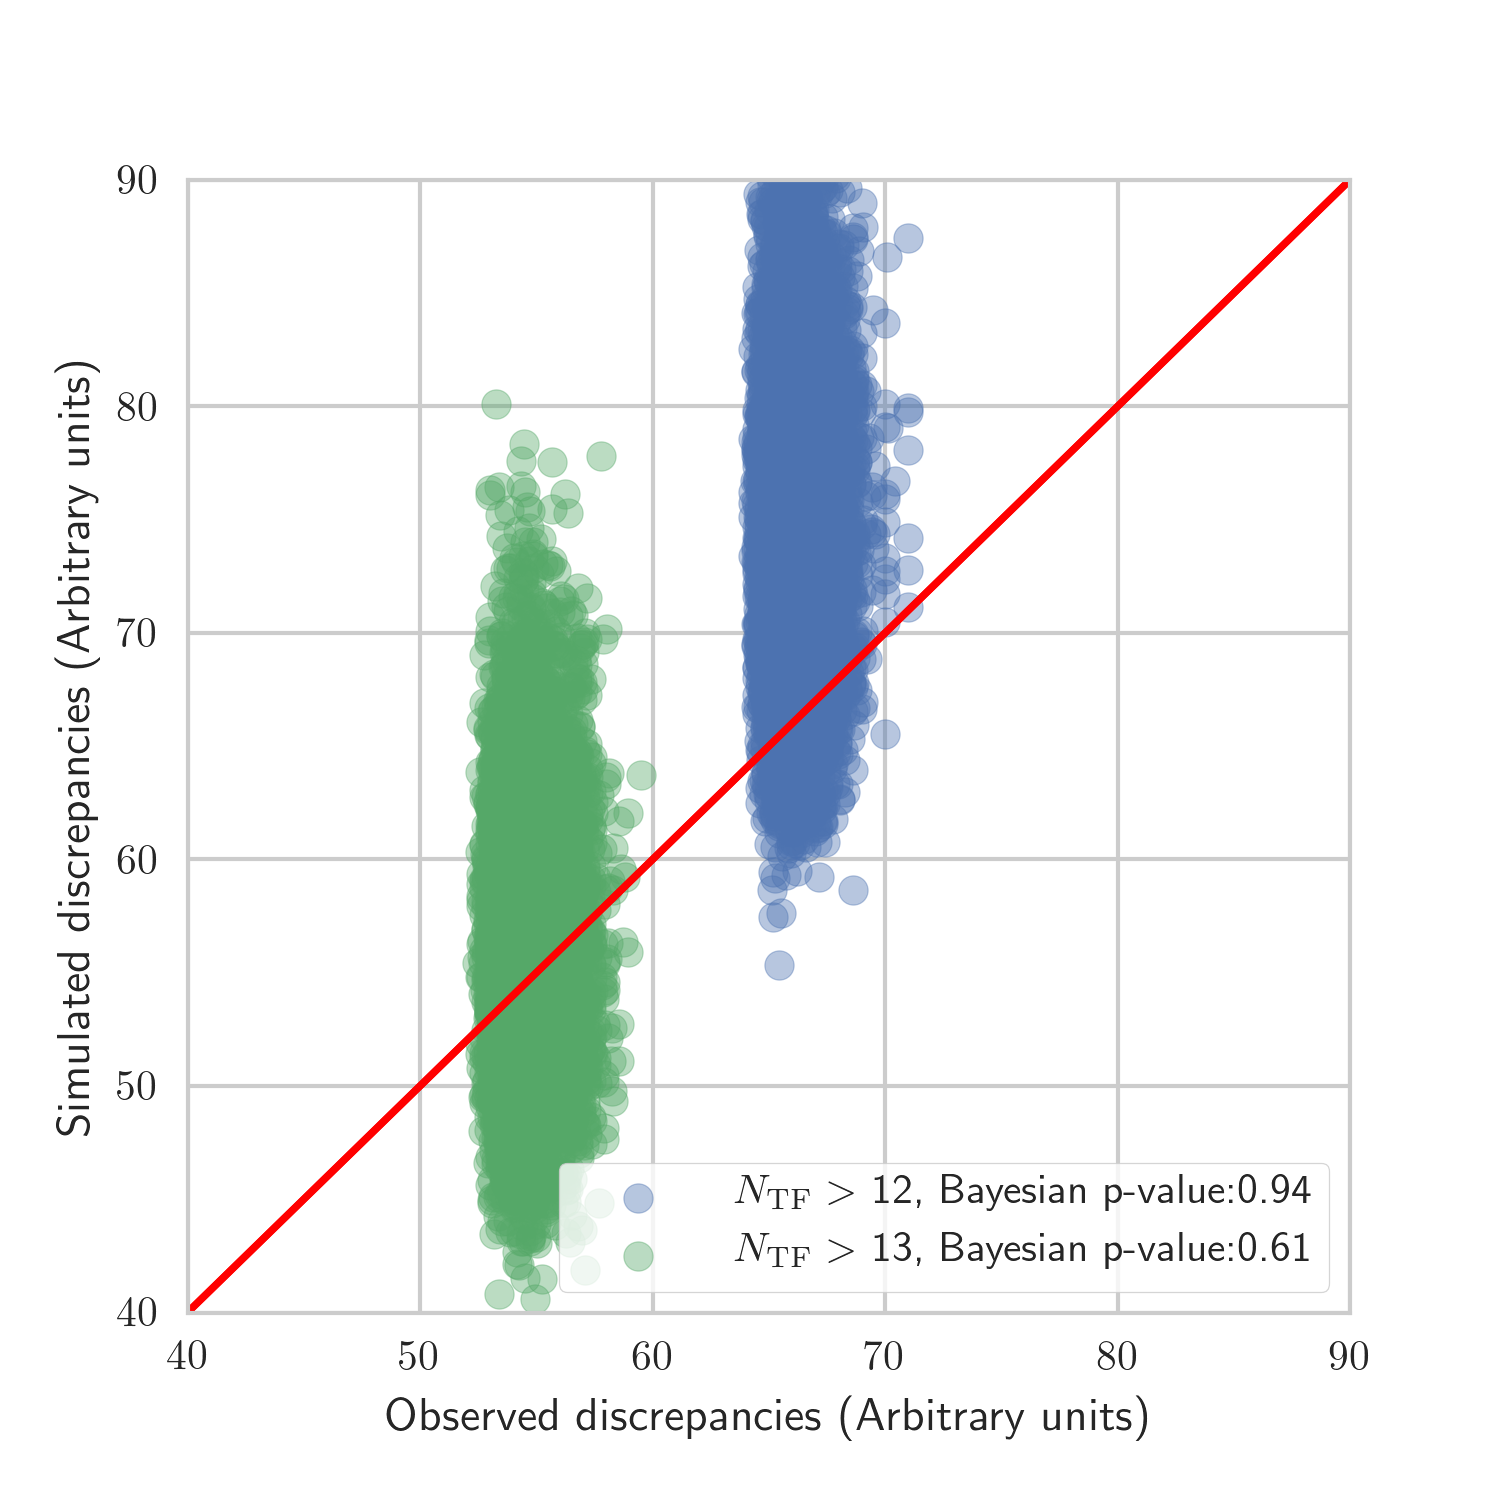
\includegraphics[scale=0.7]{discq2.png}
    \caption{Discrepancy plot for the Bayesian quadrature model (equation~\ref{eq:bayq}) based on errors estimated using method M. }
    \label{fig:discq2}
\end{figure*}
\begin{figure*}
	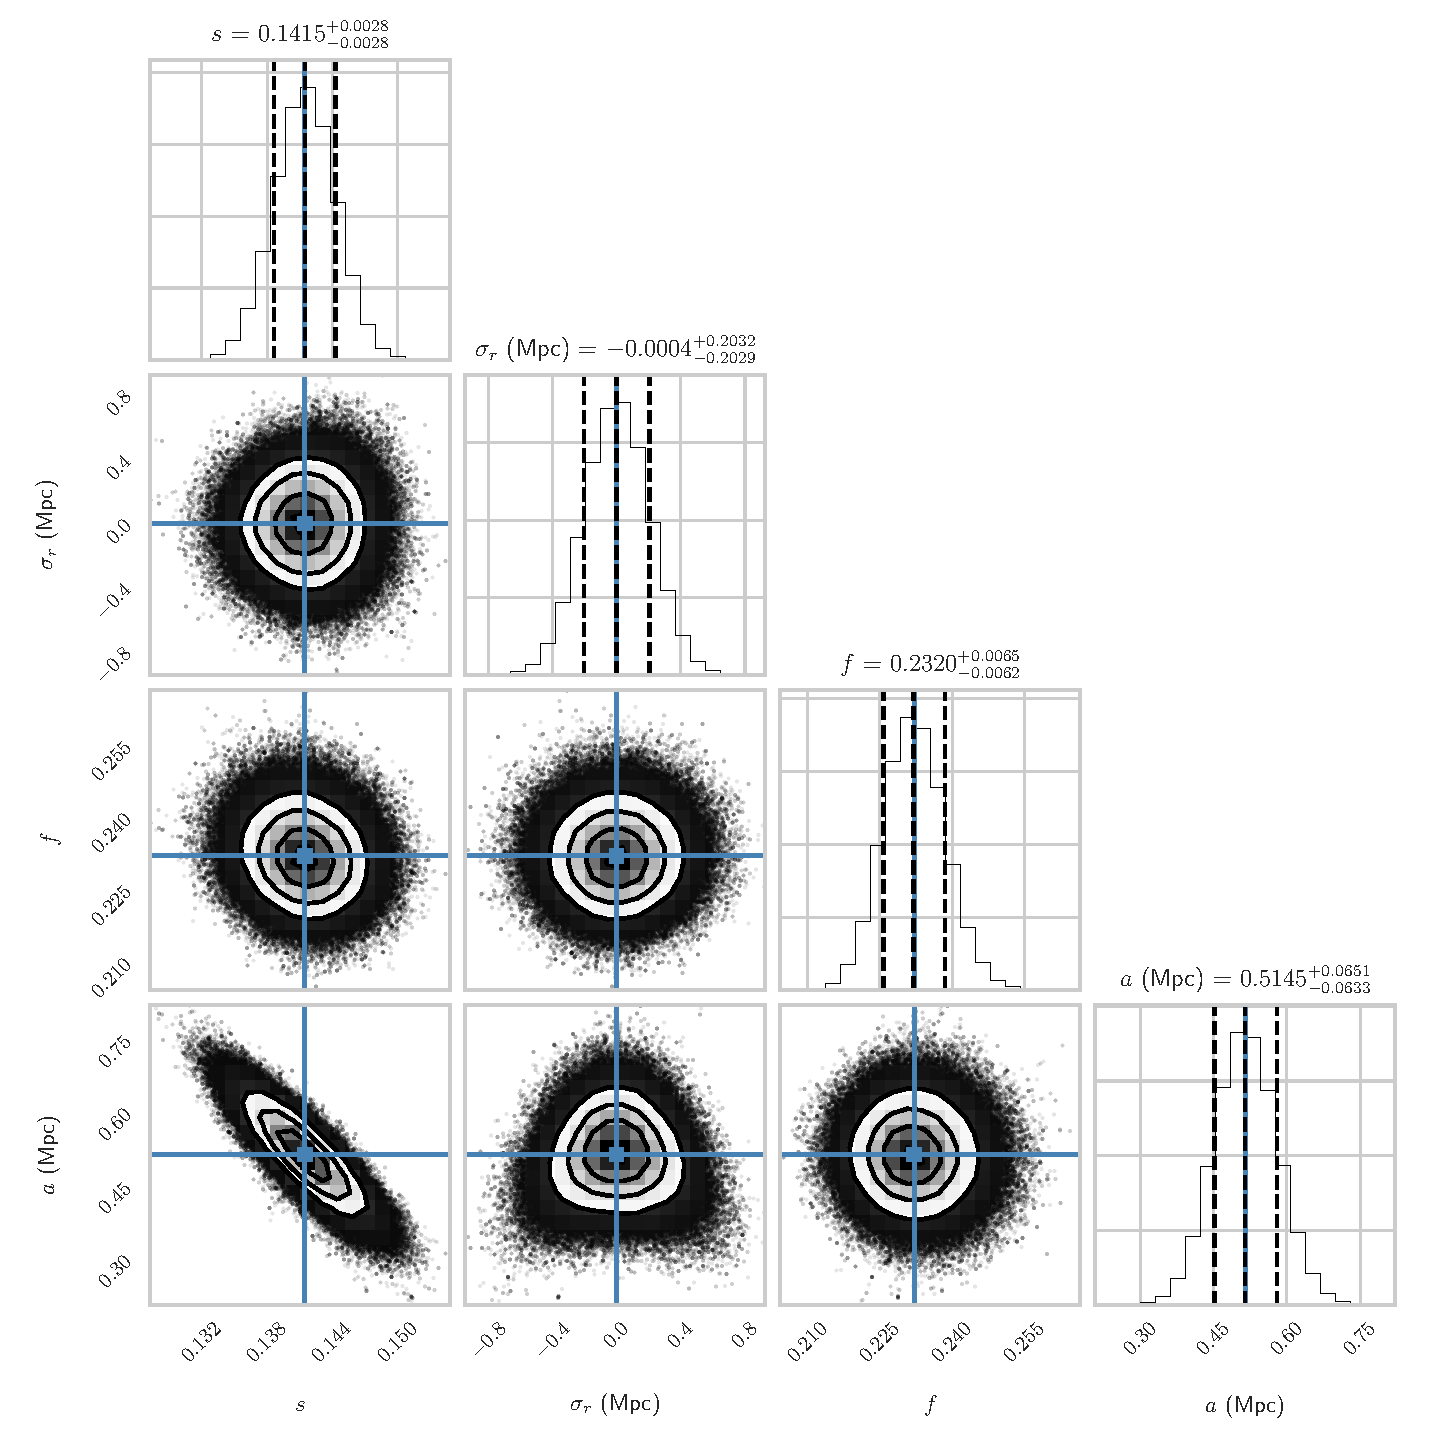
\includegraphics[scale=0.7]{cornerq2}
    \caption{Corner plot showing the \texttt{emcee} sampling of the posterior probability distribution (equation \ref{eq:ppd}) for the quadrature Bayesian model parameters $\pmb{\theta}=(s,\sigma_r,f,a)$ based on errors estimated using method M for galaxies with more than 13 TF distance measurements. The dashed lines indicate the 16th, 50th, and 84th percentile of the marginalized distribution of each parameter (shown at the top of each column), and the blue solid lines indicate the mean. This plot was made using the \texttt{corner} Python module.}
    \label{fig:cornerq2}
\end{figure*}
\begin{figure*}
	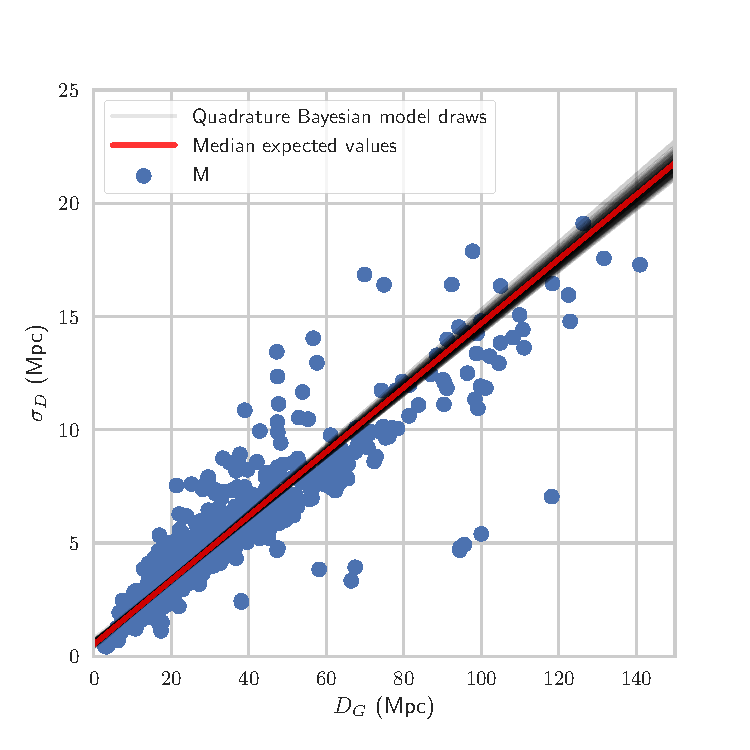
\includegraphics[scale=0.7]{drawsq2}
    \caption{Projection of parameter set samples from the posterior probability distribution of the Bayesian quadrature model onto the $D_G$ vs. $\sigma_D$ scatter plot for errors estimated using method M for galaxies with more than 13 TF distance measurements.}
    \label{fig:drawsq2}
\end{figure*}
\subsection{Bayesian Linear Model}
\label{sec:blm}
In Section~\ref{sec:bqm} above we conclude that we can ignore the random error component in equation~\ref{eq:bayq} in order to work with a simpler, numerically stable, linear model that only considers a systematic error with scale factor and zero setting error components,
\begin{equation}
\sigma_D=\sigma_s=sD+a\ .
	\label{eq:bayl}
\end{equation}
We also update our prior considering that the quadratic model yielded lower values for the zero setting error $a$ than previously considered in equation~\ref{eq:priorq},
\begin{equation}
P(s,a,\sigma_r)=\left\{
\begin{aligned}
1,\ \ \ \ &\mathrm{if}\ \ \ 0<s<1\ \mathrm{and}\\
& \ \ \ \ \  0<a<2\ \mathrm{Mpc}\ \mathrm{and}\\
& \ \ \ \ \  0<f<1\\
0,\ \ \ \ &\ \mathrm{otherwise.}
\end{aligned}
\right.
\end{equation}
We use \texttt{emcee} to sample the posterior over $\pmb{\theta}=(s,a,f)$ using 100 walkers and 10000 steps ($t_\mathrm{autocorr} < 50$ steps) for the linear Bayesian model applied to H errors. The discrepancy plot (Fig.~\ref{fig:discl}) shows a significant improvement over the quadratic model, as it shows an acceptable Bayesian $p$-value for the 473 galaxies with $N>15$ measurements (9259 in total), whereas the quadratic model replicated errors only for galaxies with $N>25$ measurements. Fig.~\ref{fig:cornerl}, shows that for the linear Bayesian model using H errors for galaxies with more than 15 measurements, $s=0.200_{-0.006}^{+0.006}$, $a=0.76_{-0.12}^{+0.13}$ Mpc, and $f=0.256_{-0.009}^{+0.009}$.
\begin{figure*}
	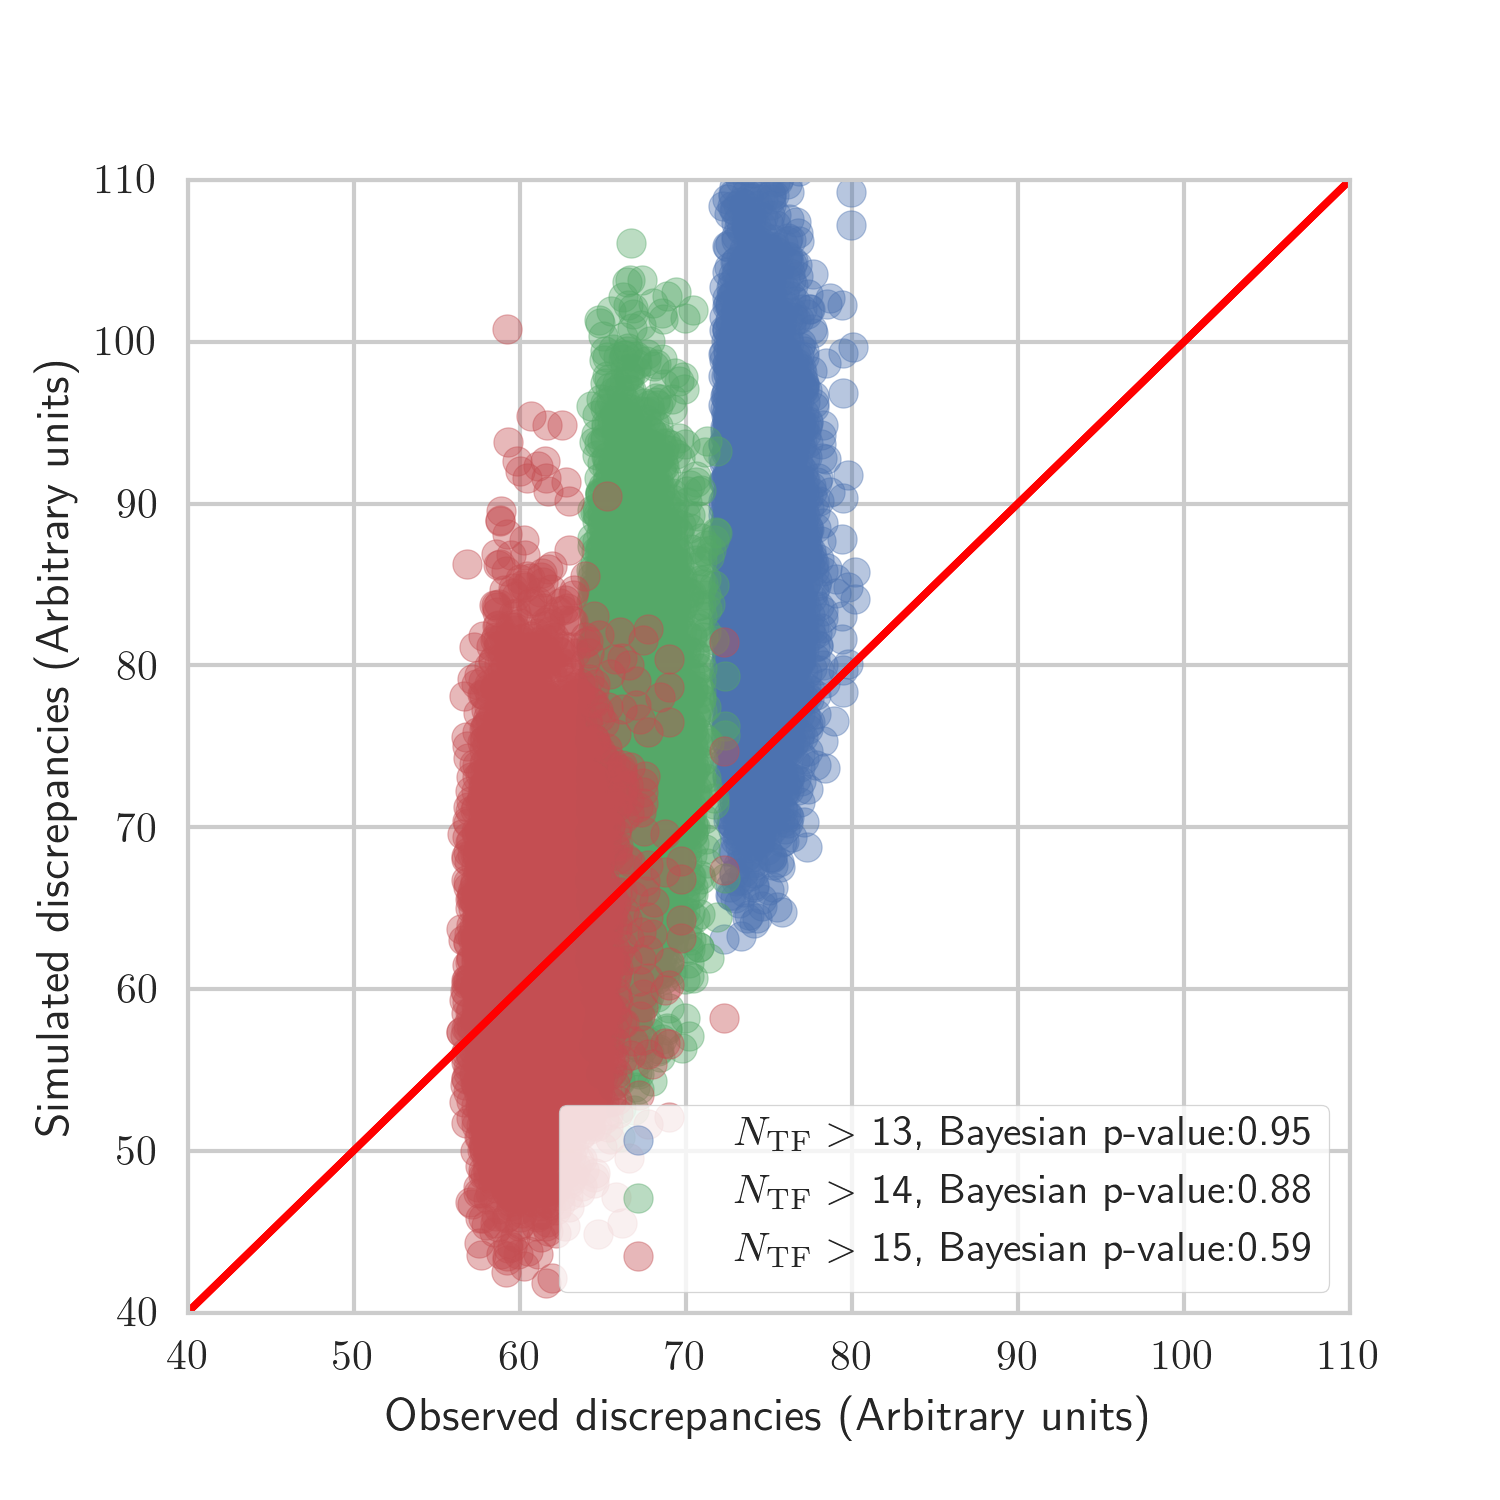
\includegraphics[scale=0.7]{discl.png}
    \caption{Discrepancy plot for the Bayesian linear model (equation~\ref{eq:bayl}) based on errors estimated using method H. }
    \label{fig:discl}
\end{figure*}
\begin{figure*}
	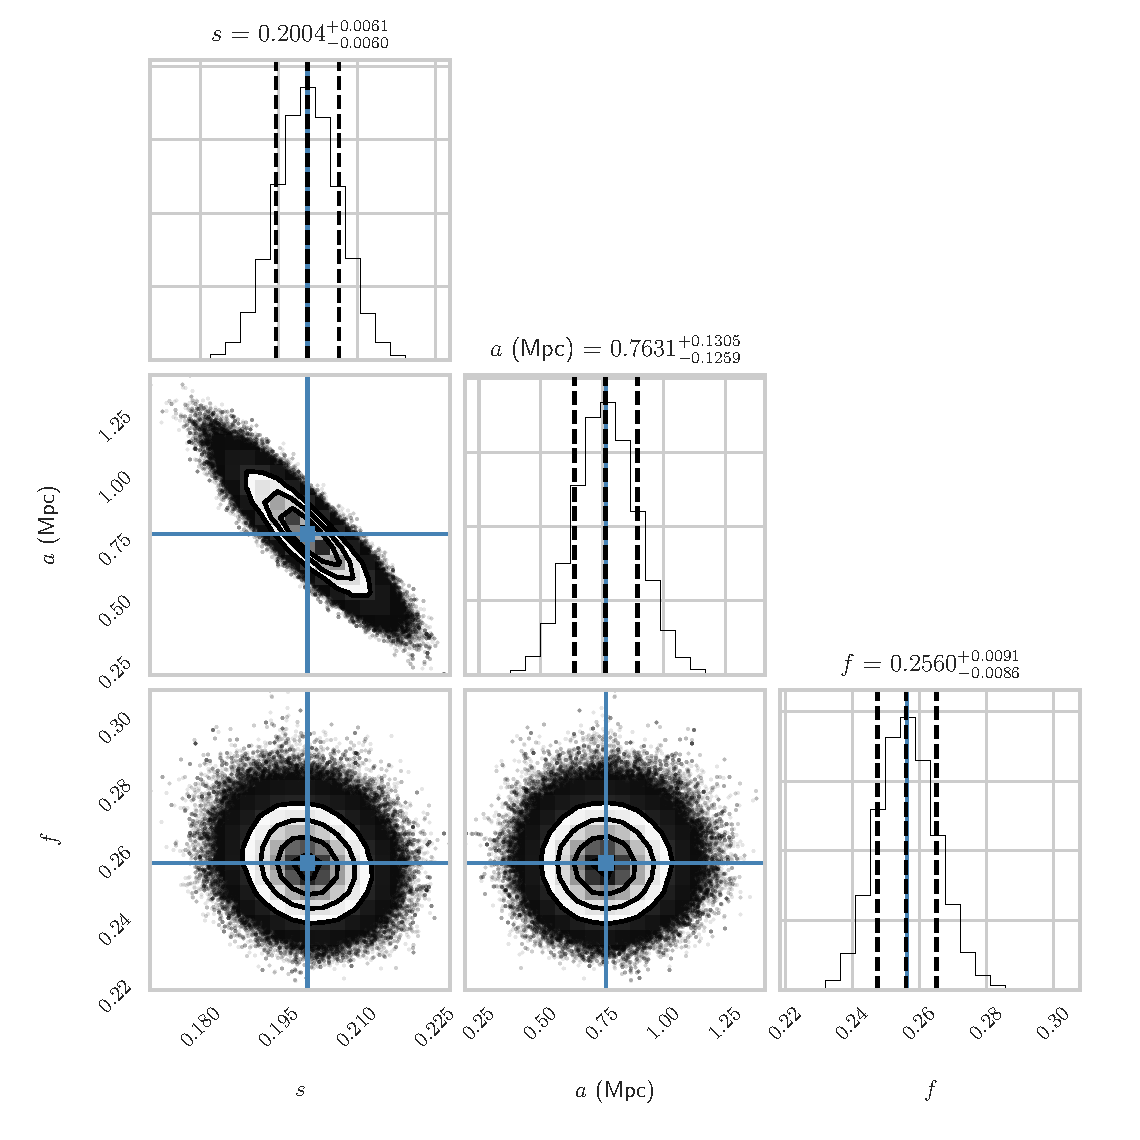
\includegraphics[scale=0.7]{cornerl}
    \caption{Corner plot showing the \texttt{emcee} sampling of the posterior probability distribution (equation \ref{eq:ppd}) for the linear Bayesian model parameters $\pmb{\theta}=(s,a,f)$ based on errors estimated using method H for galaxies with more than 15 TF distance measurements. The dashed lines indicate the 16th, 50th, and 84th percentile of the marginalized distribution of each parameter (shown at the top of each column), and the blue solid lines indicate the mean. This plot was made using the \texttt{corner} Python module.}
    \label{fig:cornerl}
\end{figure*}
We sample the posterior for the linear model applied to M errors using \texttt{emcee} with 100 walkers and 10000 steps ($t_\mathrm{autocorr} < 50$ steps). Fig.~\ref{fig:discl2} shows the discrepancy plot, which does not show a significant improvement of the linear over the quadratic model for M errors, as it also works for galaxies with $N>13$ measurements. This happens because the sampling of the posterior for the quadratic model (Fig.~\ref{fig:cornerq2}) does not show a degeneracy between $\sigma_r$ and $a$, and also because the marginalized posterior distribution for $\sigma r$ is a near-zero distribution with a variance of $0.2$ Mpc. The parameters according the the linear model and data are $s=0.142_{-0.003}^{+0.003}$, $a=0.53_{-0.06}^{+0.06}$ Mpc, and $f=0.228_{-0.006}^{+0.006}$, as shown in Fig.~\ref{fig:cornerl2}. 
\begin{figure*}
	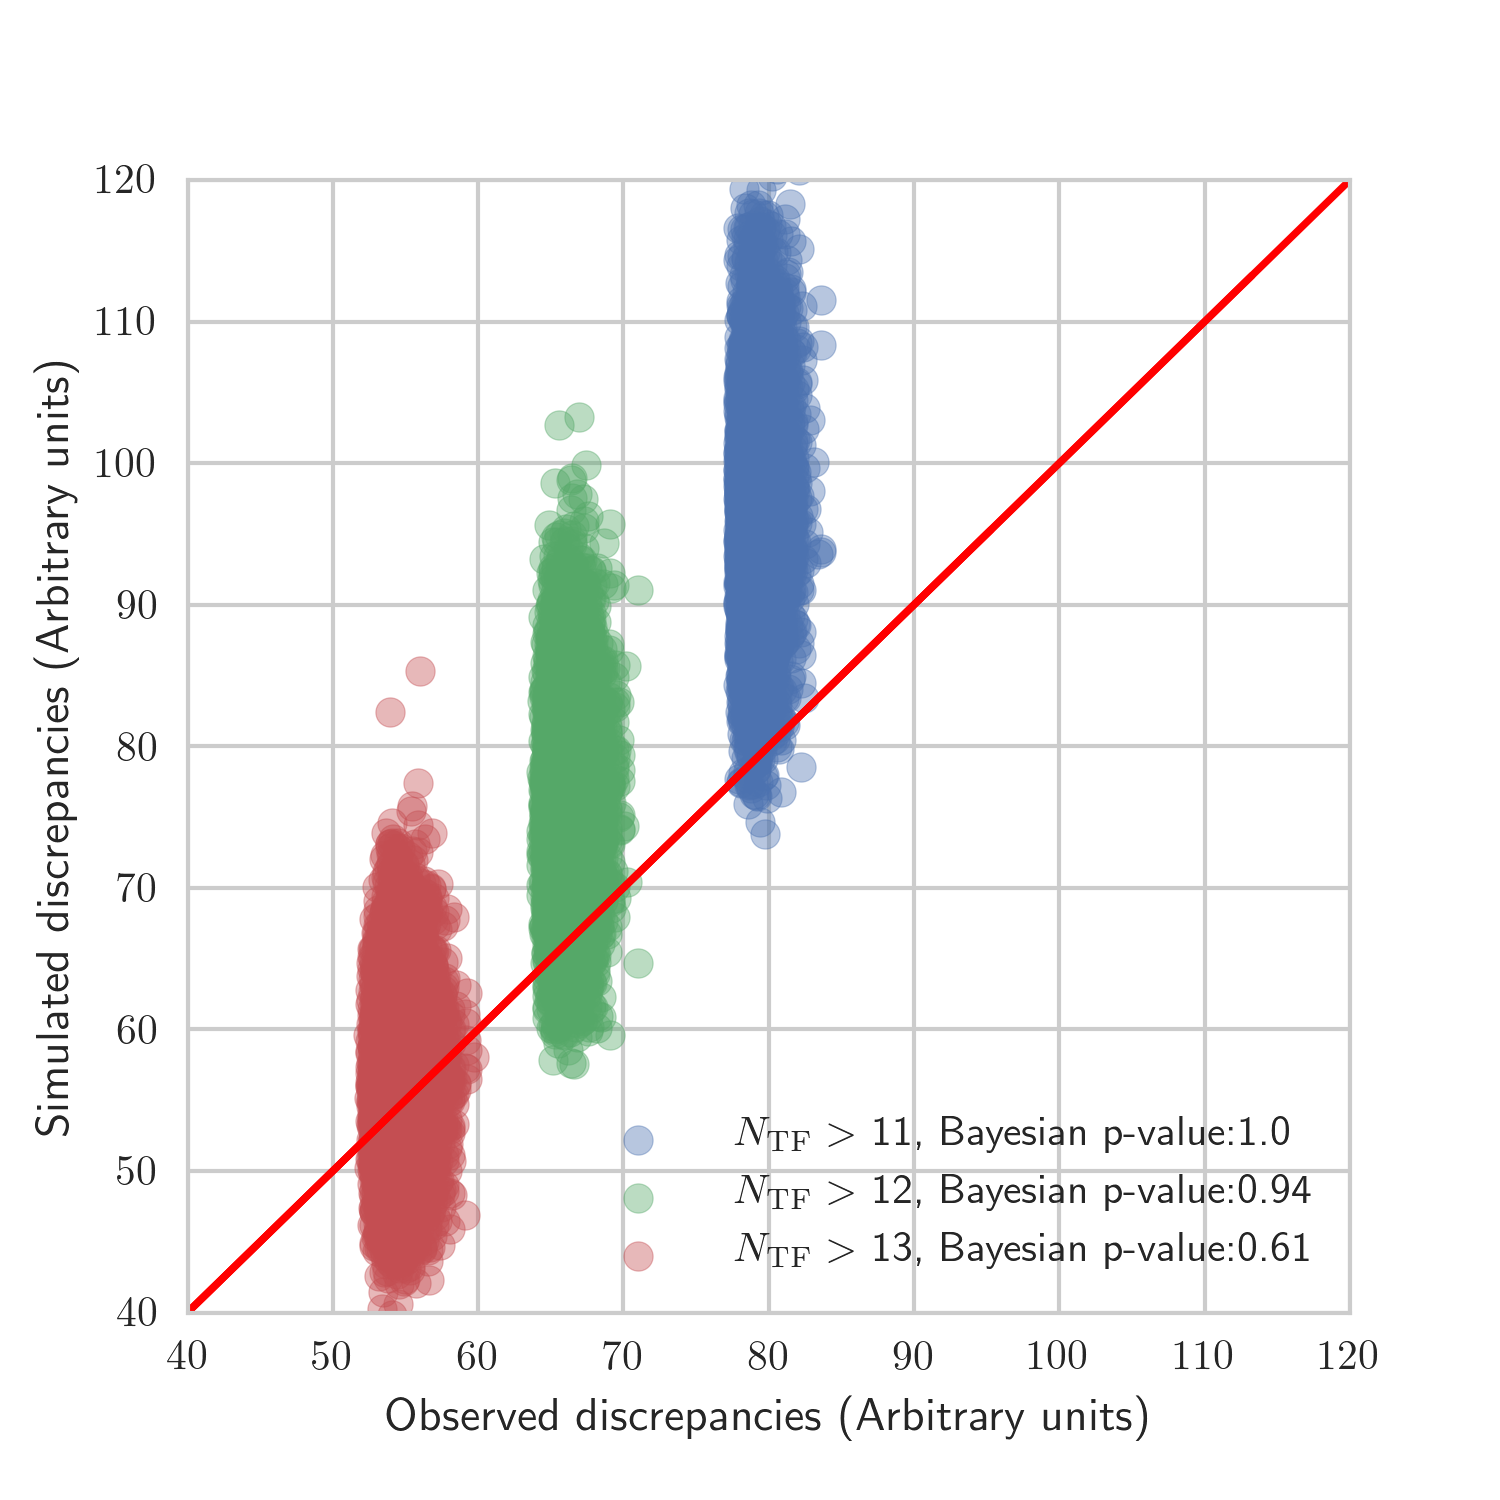
\includegraphics[scale=0.7]{discl2.png}
    \caption{Discrepancy plot for the Bayesian linear model (equation~\ref{eq:bayl}) based on errors estimated using method M. }
    \label{fig:discl2}
\end{figure*}
\begin{figure*}
	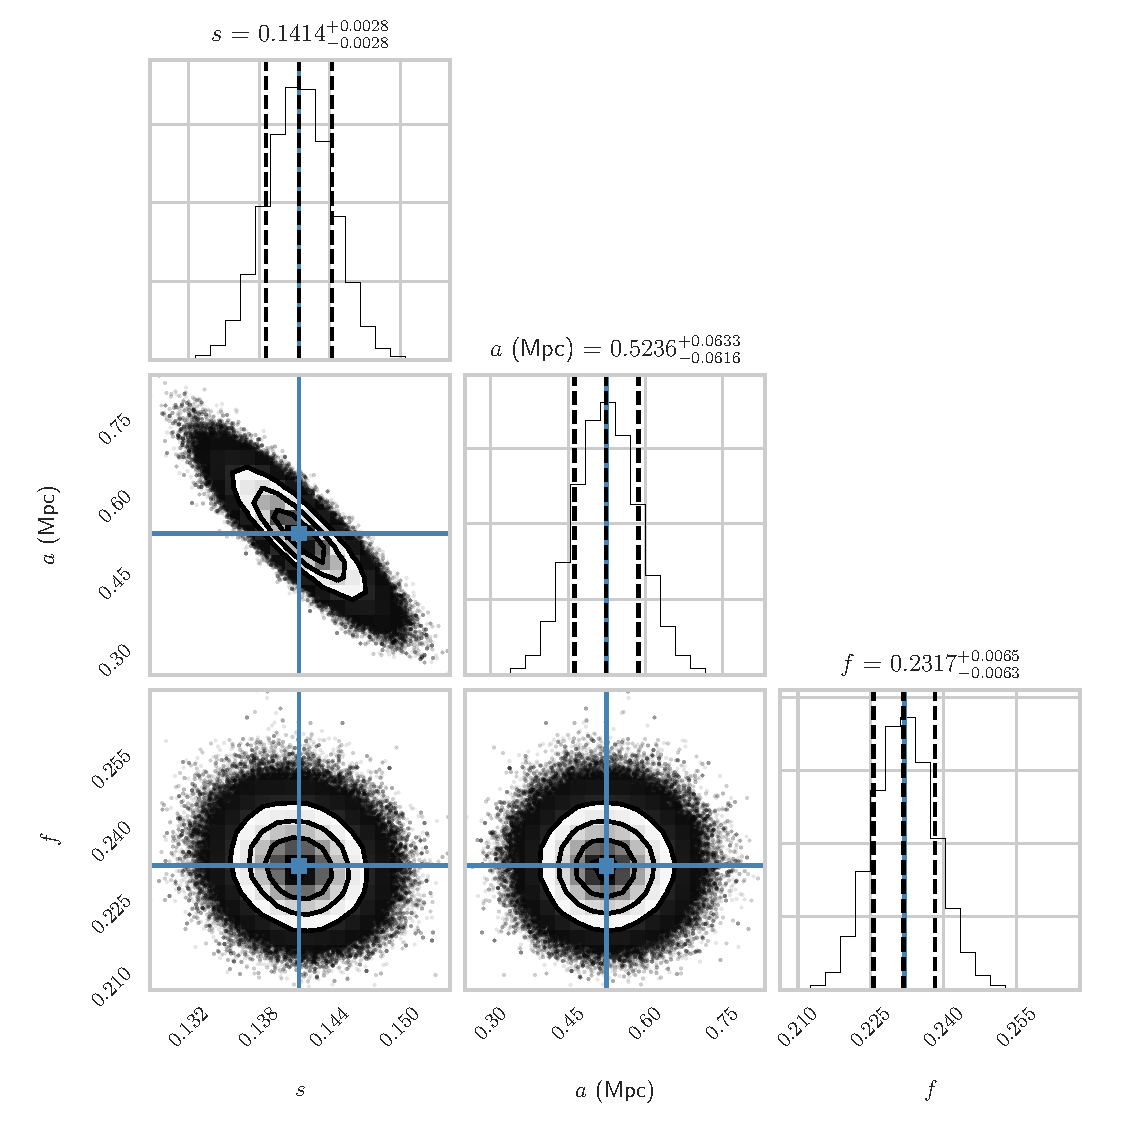
\includegraphics[scale=0.7]{cornerl2}
    \caption{Corner plot showing the \texttt{emcee} sampling of the posterior probability distribution (equation \ref{eq:ppd}) for the linear Bayesian model parameters $\pmb{\theta}=(s,a,f)$ based on errors estimated using method M for galaxies with more than 13 TF distance measurements. The dashed lines indicate the 16th, 50th, and 84th percentile of the marginalized distribution of each parameter (shown at the top of each column), and the blue solid lines indicate the mean. This plot was made using the \texttt{corner} Python module.}
    \label{fig:cornerl2}
\end{figure*}
\begin{figure*}
	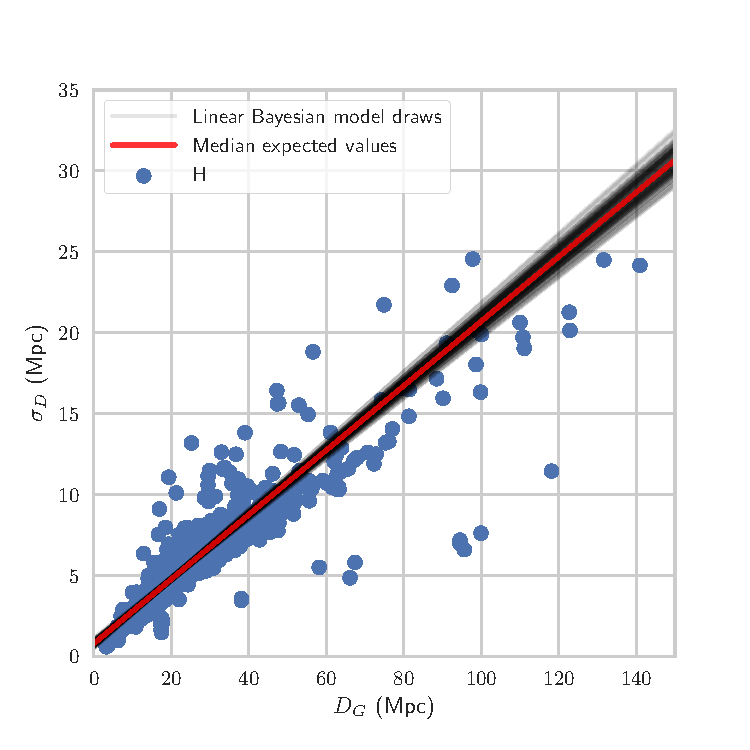
\includegraphics[scale=0.7]{drawsl}
    \caption{Projection of parameter set samples from the posterior probability distribution of the Bayesian linear model onto the $D_G$ vs. $\sigma_D$ scatter plot for errors estimated using method H for galaxies with more than 15 TF distance measurements.}
    \label{fig:drawsl}
\end{figure*}
\begin{figure*}
	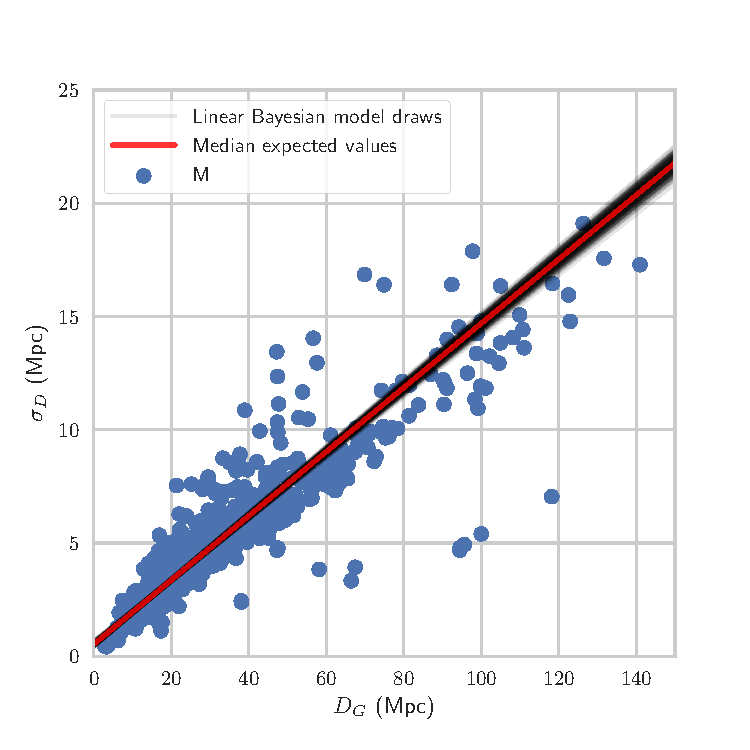
\includegraphics[scale=0.7]{drawsl2}
    \caption{Projection of parameter set samples from the posterior probability distribution of the Bayesian linear model onto the $D_G$ vs. $\sigma_D$ scatter plot for errors estimated using method M for galaxies with more than 13 TF distance measurements.}
    \label{fig:drawsl2}
\end{figure*}
\begin{figure*}
	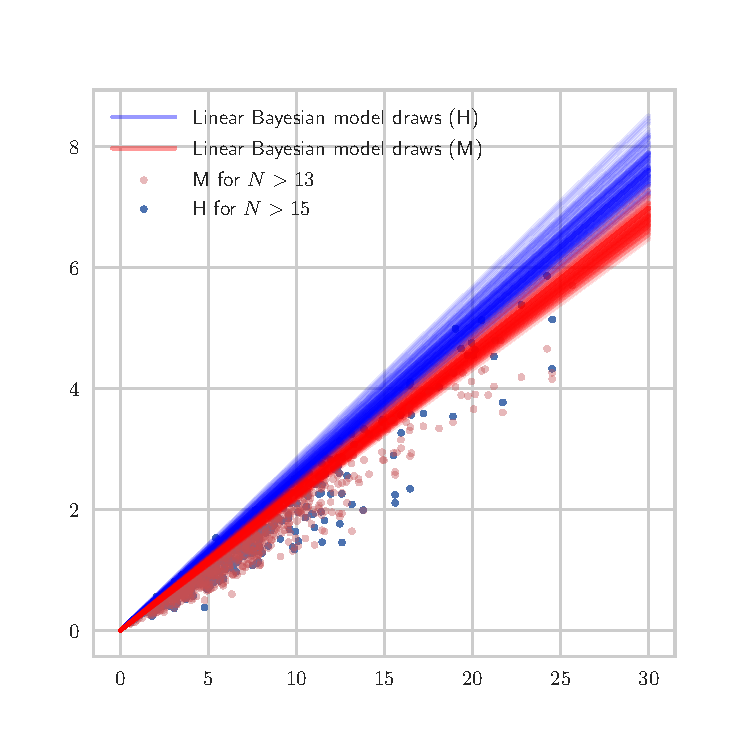
\includegraphics[scale=0.7]{drawsee}
    \caption{Projection of parameter set samples from the posterior probability distribution of the Bayesian linear model onto the $\sigma_D$ vs. $\sigma_\sigma$ scatter plot for errors estimated using methods H and M for galaxies with more than 15 and 13 TF distance measurements, respectively.}
    \label{fig:drawsee}
\end{figure*}
\subsection{Predictions for missing errors}
\label{sec:pred} 
Our linear Bayesian model is able to predict the intrinsic variance of H and M errors by modeling them as systematic errors, with zero setting and scale factor error components. The lower limit of distance measurements for which the model works for H and M errors, is 15 and 13, respectively. Figs.~\ref{fig:drawsl} and \ref{fig:drawsl2} respectively show the linear model draws for H and M errors, for which the working range is approximately $D_G\in(3,140)$ Mpc. We also show in Fig.~\ref{fig:drawsee} that the model draws for $f$ the scale parameter for the variance of $\sigma_D$ fit the bootstrap variance of H and M errors well. Given that galaxies with the lower limit of observations quoted above are not instrinsically different to other galaxies in this range, we use the posterior predictive distribution of the linear Bayesian model for predicting errors for the 818 galaxies in NED-D for which all TF measurements lack a reported error. Figs.~\ref{fig:predl1} and \ref{fig:predl2} show synthetic errors generated from the posterior predictive distribution for the $\sigma_D$ linear model, along with the expected values of $\sigma_D$ using the median of the posterior probability distribution in equation~\ref{eq:ppd}, and the $D_G$ vs. $\sigma_D$ points for galaxies with more than 5 TF distance measurements (for contrast) for methods H and M, respectively. The median expected values are only drawn for points within the predictive range of each model, and synthetic predicted errors for galaxies outside of this range are plotted in black. The distance was calculated using the median of the reported distances whenever there was more than one TF distance measurement.% FP low number of meas per galaxy, can make a predictive model but it's not trustworthy. 
\begin{figure*}
	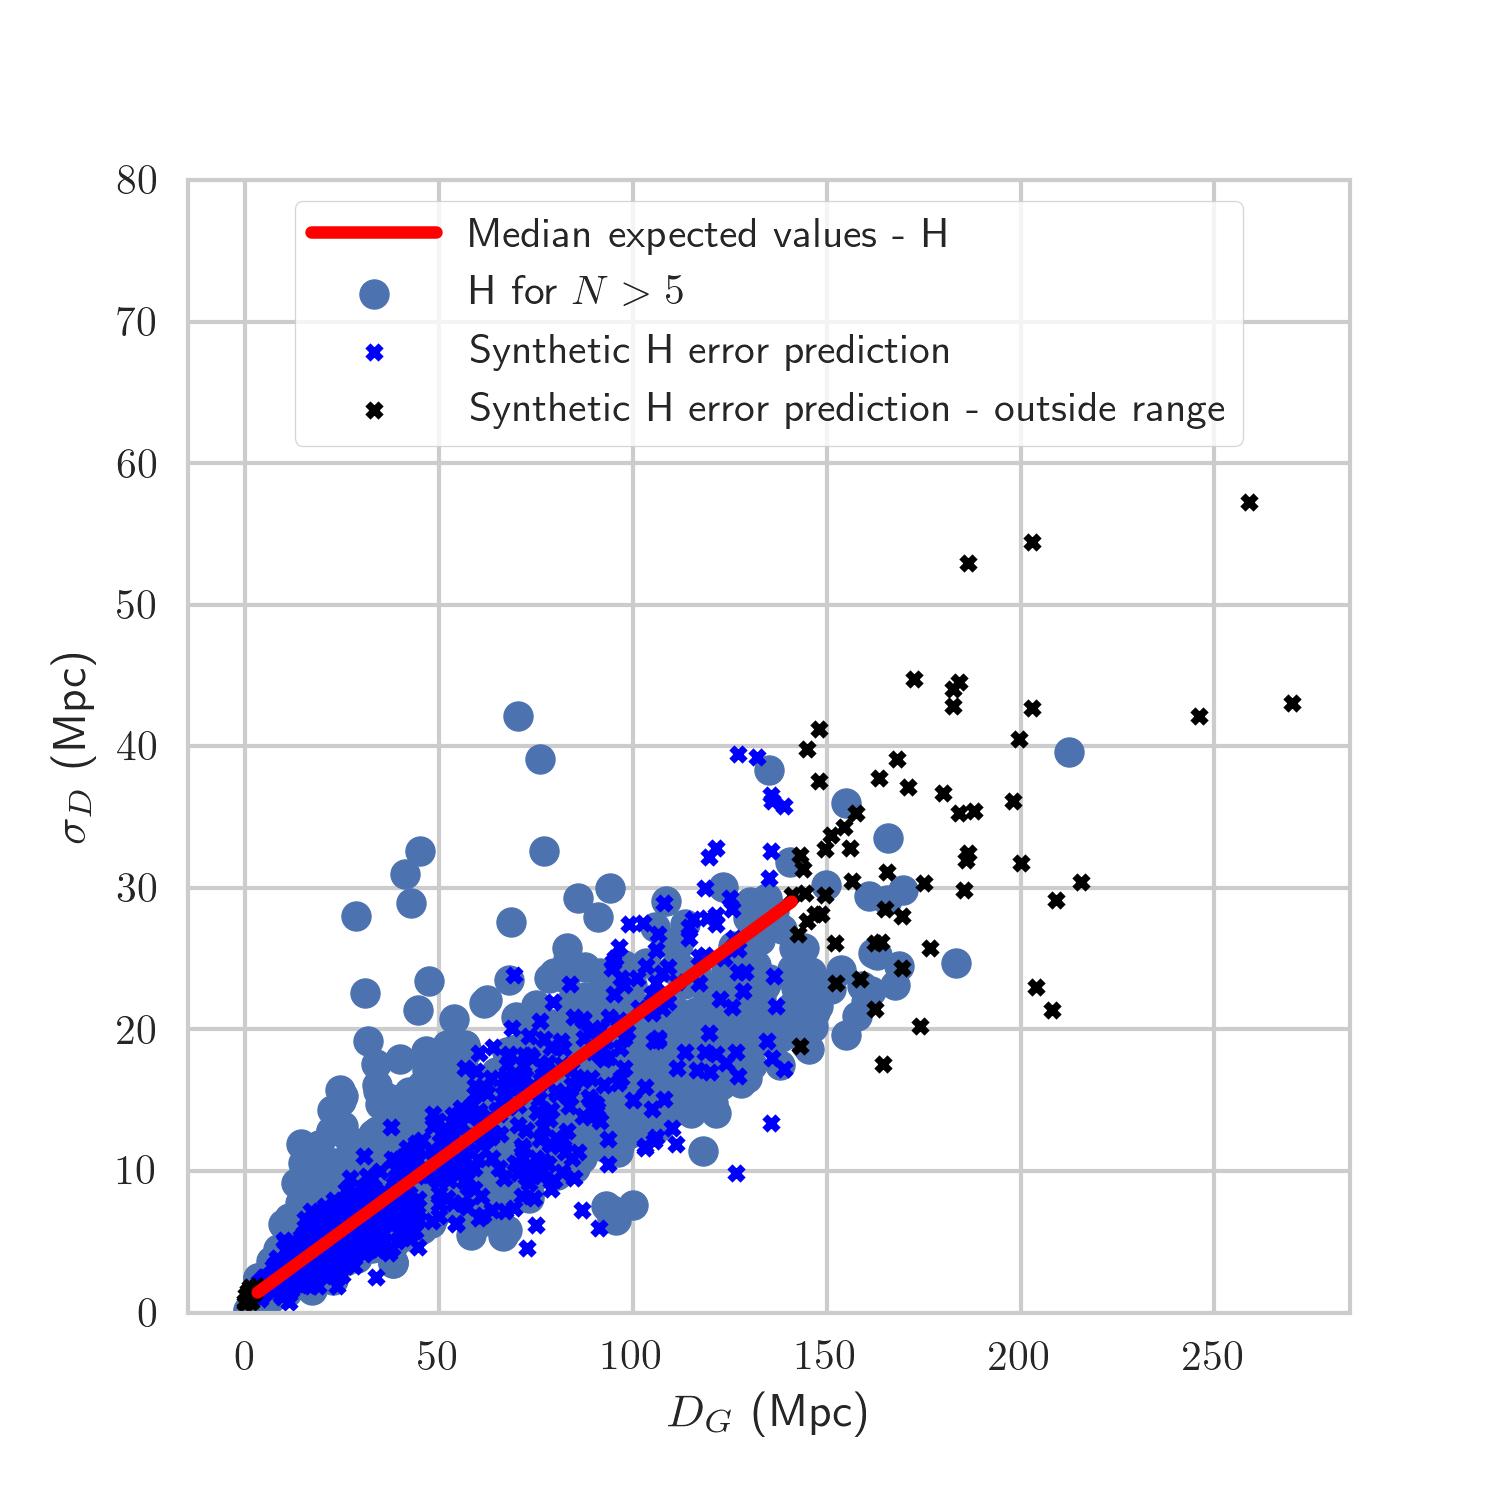
\includegraphics[scale=0.7]{predl1.png}
    \caption{Synthetic H-method $\sigma_D$ and their median expected values for the 818 galaxies in NED-D for which no TF distance measurements report an error, generated using the corresponding Bayesian linear model. Predicted errors for galaxies outside of the working distance range of the model are plotted in black. H errors for galaxies with more than 5 TF measurements are also plotted for comparison.}
    \label{fig:predl1}
\end{figure*}
\begin{figure*}
	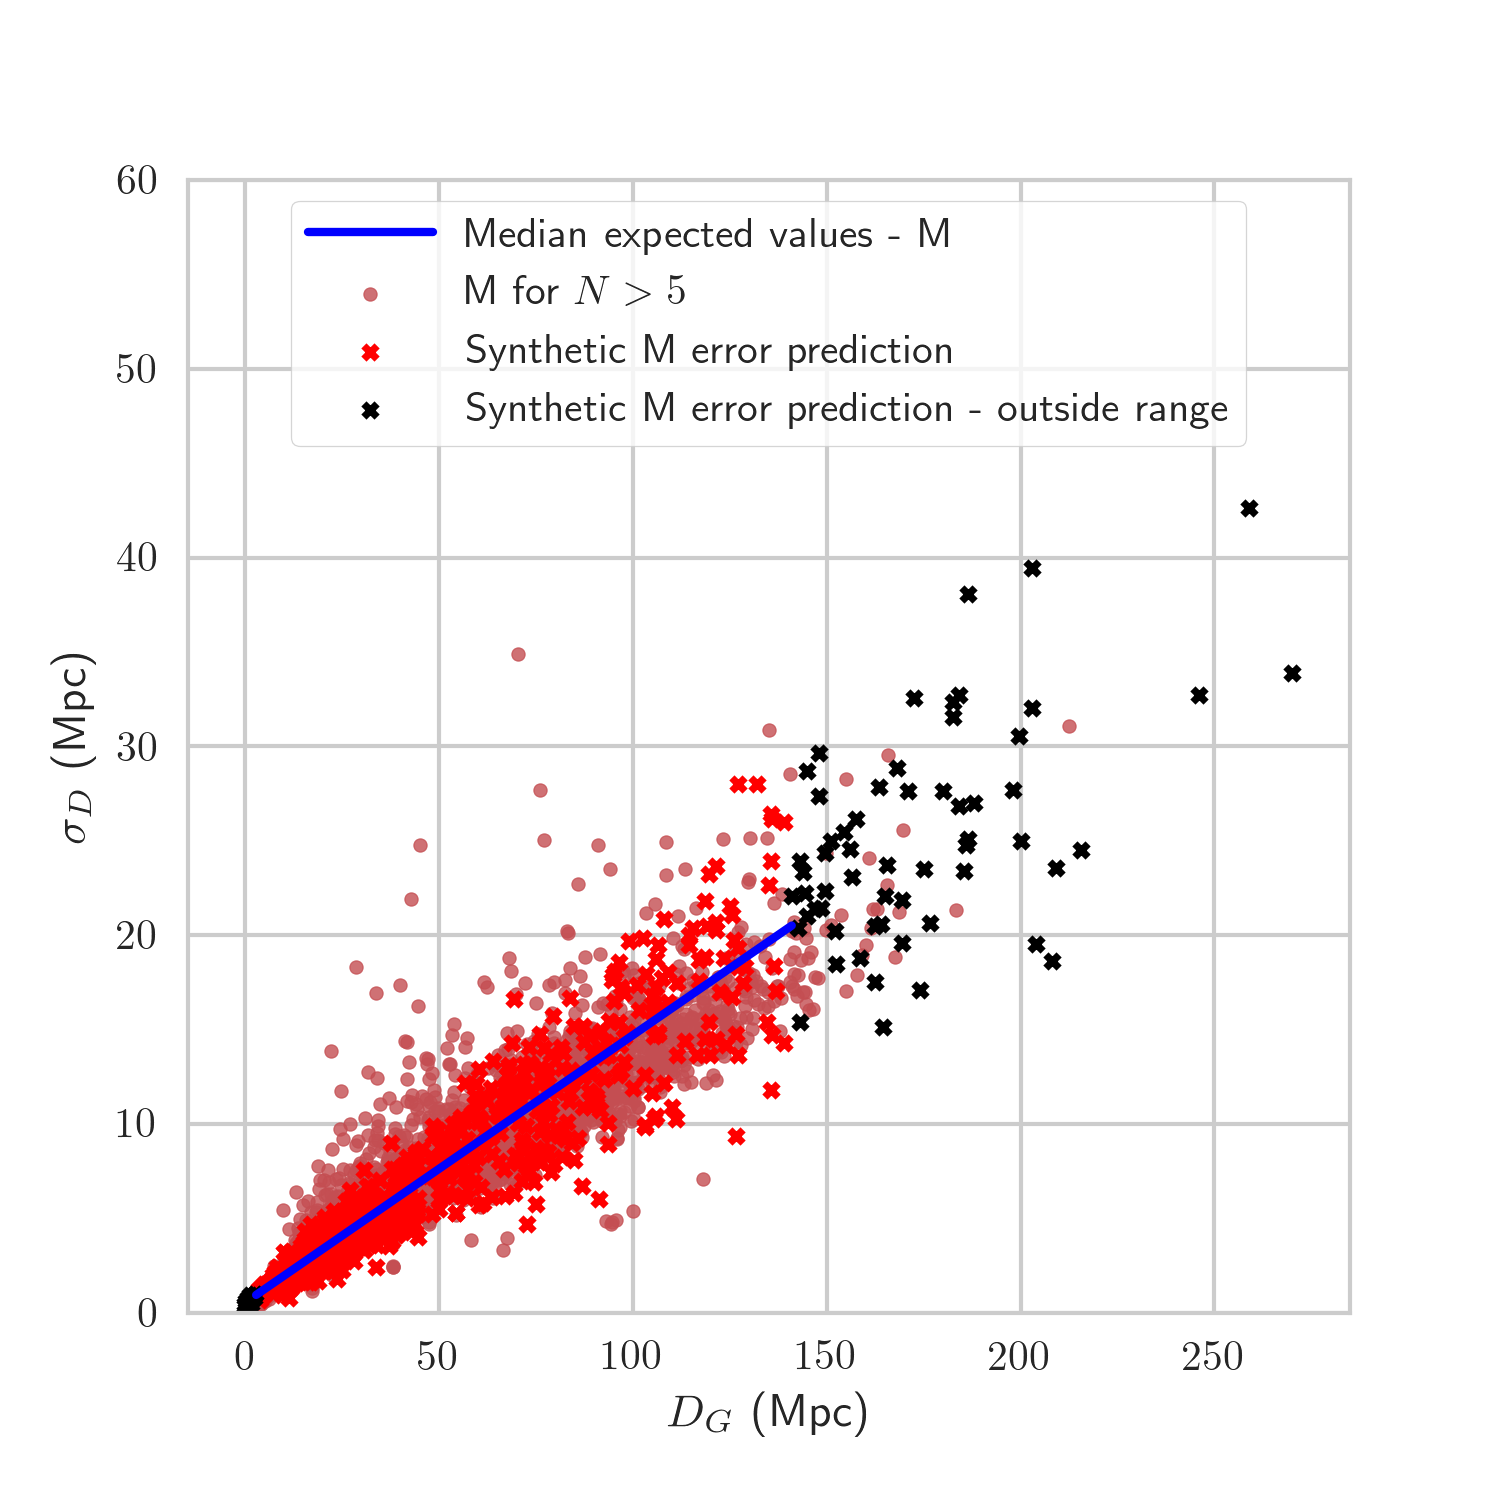
\includegraphics[scale=0.7]{predl2.png}
    \caption{Synthetic M-method $\sigma_D$ and their median expected values for the 818 galaxies in NED-D for which no TF distance measurements report an error, generated using the corresponding Bayesian linear model. Predicted errors for galaxies outside of the working distance range of the model are plotted in black. M errors for galaxies with more than 5 TF measurements are also plotted for comparison.}
    \label{fig:predl2}
\end{figure*}

\section{Conclusions}

Discrepancy plots should be more widely used. 

\section*{Acknowledgements}

The authors would like to thank O. L. Ram\'irez-Su\'arez and J. E. Forero-Romero for their valuable input during the early stages of this work. This research has made use of the NASA/IPAC Extragalactic Database (NED), which is operated by the Jet Propulsion Laboratory, California Institute of Technology, under contract with the National Aeronautics and Space Administration.

%%%%%%%%%%%%%%%%%%%%%%%%%%%%%%%%%%%%%%%%%%%%%%%%%%

%%%%%%%%%%%%%%%%%%%% REFERENCES %%%%%%%%%%%%%%%%%%

% The best way to enter references is to use BibTeX:

\bibliographystyle{mnras}
\bibliography{savedrecs} % if your bibtex file is called example.bib


% Alternatively you could enter them by hand, like this:
% This method is tedious and prone to error if you have lots of references
%\begin{thebibliography}{99}
%\bibitem[\protect\citeauthoryear{Author}{2012}]{Author2012}
%Author A.~N., 2013, Journal of Improbable Astronomy, 1, 1
%\bibitem[\protect\citeauthoryear{Others}{2013}]{Others2013}
%Others S., 2012, Journal of Interesting Stuff, 17, 198
%\end{thebibliography}

%%%%%%%%%%%%%%%%%%%%%%%%%%%%%%%%%%%%%%%%%%%%%%%%%%

%%%%%%%%%%%%%%%%% APPENDICES %%%%%%%%%%%%%%%%%%%%%

\appendix

\section{Estimation of errors for HyperLEDA}
We estimated errors for the HyperLEDA redshift-independent extragalactic distance database using the methods described in Section~\ref{sec:comp} across all distance determination methods, ignoring measurements with no reported errors. As expected from our analysis of TF errors in NED-D, errors calculated with methods P, Q, and M overpredict the error with respect to the H method for galaxies with a low number of distance measurements ($N=2$), as shown in Fig.~\ref{fig:HLlow}. Fig.~\ref{fig:HLhigh} shos that for galaxies with a higher number of distance measurements, the P method significantly underpredicts the error with respect to the other methods. Even though the H and Q methods show a similar trend, the variance of Q errors around this trend is higher than for H methods. Errors obtained with method M are lower, due to the method's intrinsic robustness. These estimations are reported in the file calles \texttt{hl\_bootstrap\_results.csv} in the repository. The fields are:
\begin{itemize}
\item \texttt{objname} - Object name according to the HyperLEDA database.
\item \texttt{j2000} - Standard epoch.
\item \texttt{meas} - Number of distance measurements.
\item \texttt{D (Mpc)} - For single distance measurements, this is the metric distance derived from the distance modulus. For $N>1$, this is the median of the posterior distribution of the corresponding extragalactic distance.
\item \texttt{H} - Error estimated using the H method. For $N=1$ this field is set to 0.
\item \texttt{M} - Error estimated using the M method. For $N=1$ this field is set to 0.
\item \texttt{P} - Error estimated using the P method. For $N=1$ this is calculated using the error propagation of the distance modulus error.
\item \texttt{Q} - Error estimated using the Q method. For $N=1$ this field is set to 0.
\end{itemize}

\begin{figure*}
	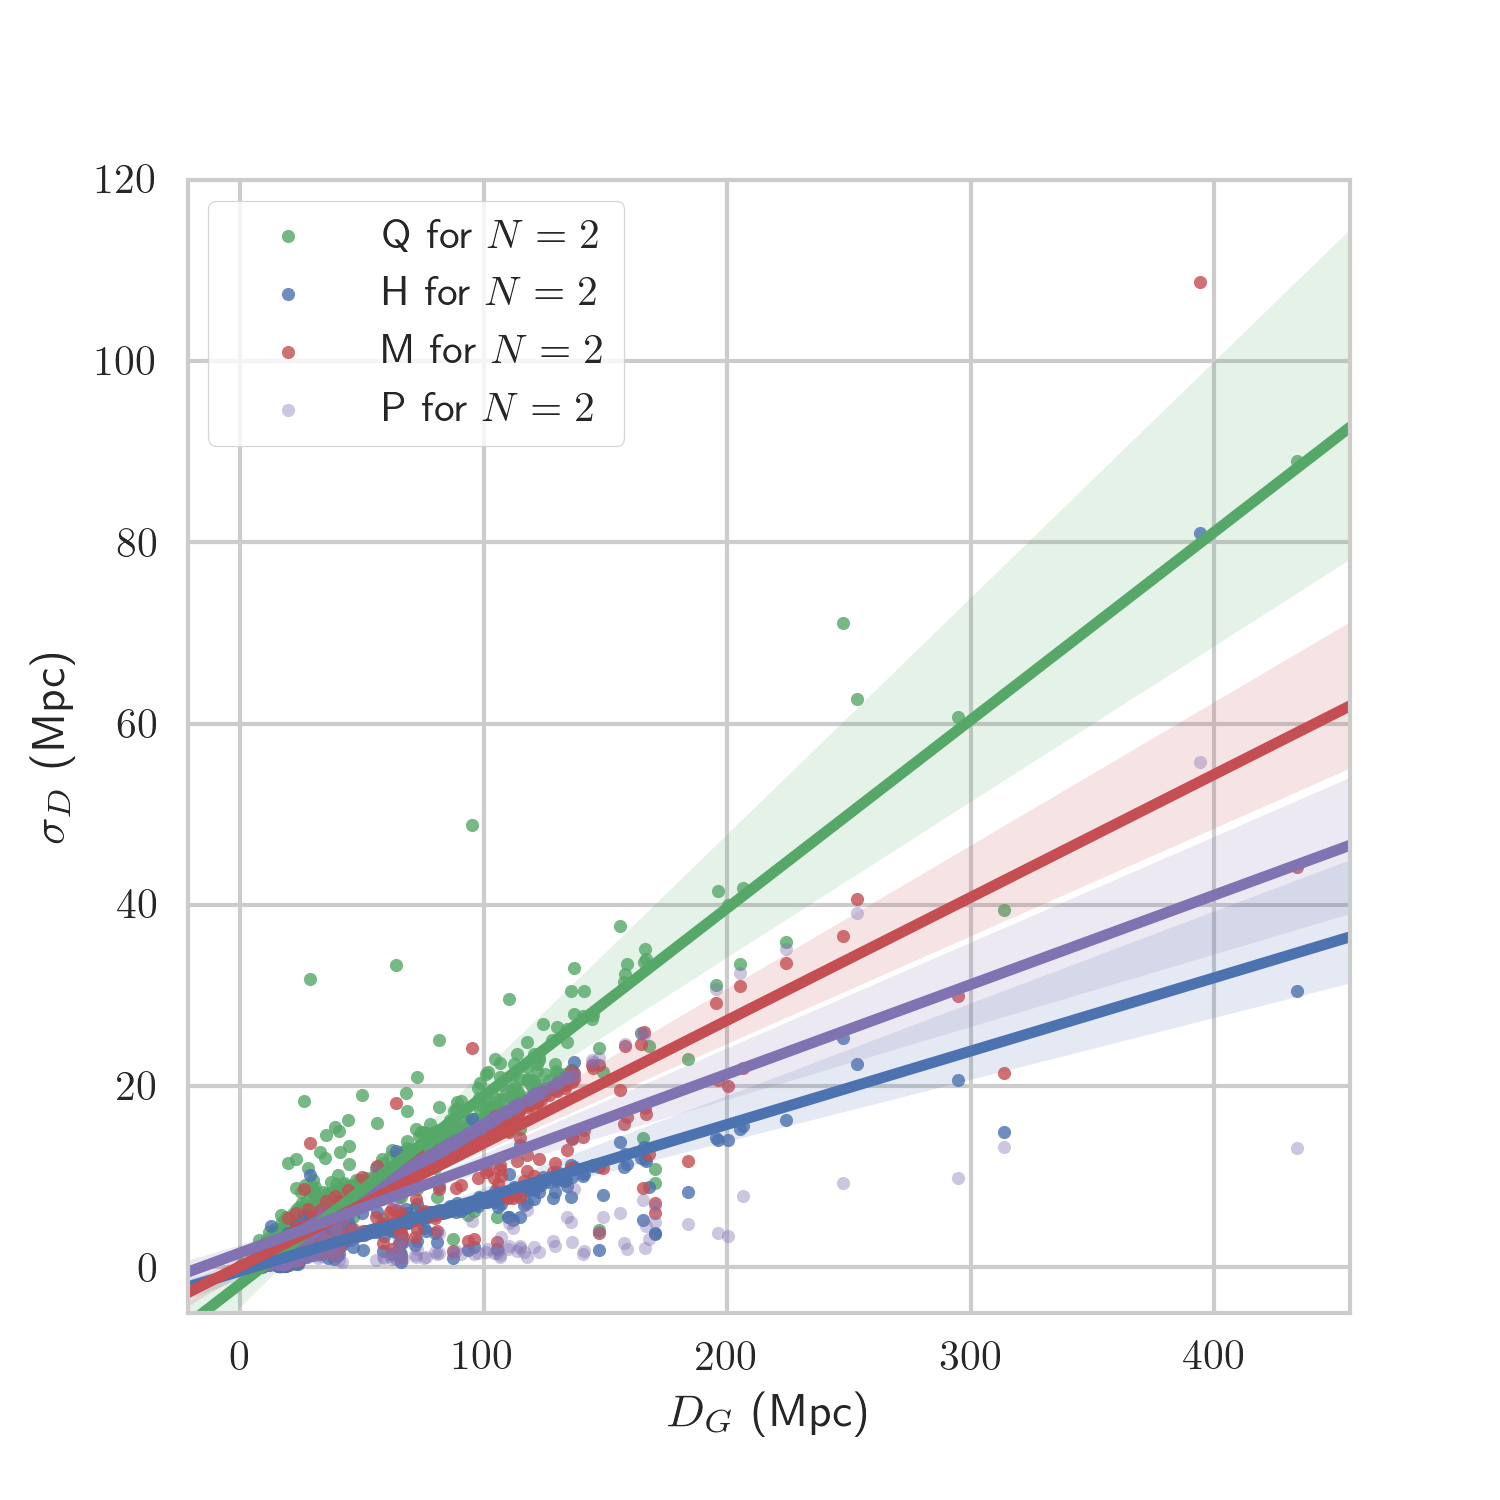
\includegraphics[scale=0.7]{HLlow.png}
    \caption{Median extragalactic distance vs. predicted extragalactic distance errors for galaxies with 2 redshift-independent distance measurements in HyperLEDA according to the H, M, Q, P error models, showing a linear regression and confidence intervals computed using the \texttt{seaborn.regplot} Python function.}
    \label{fig:HLlow}
\end{figure*}
\begin{figure*}
	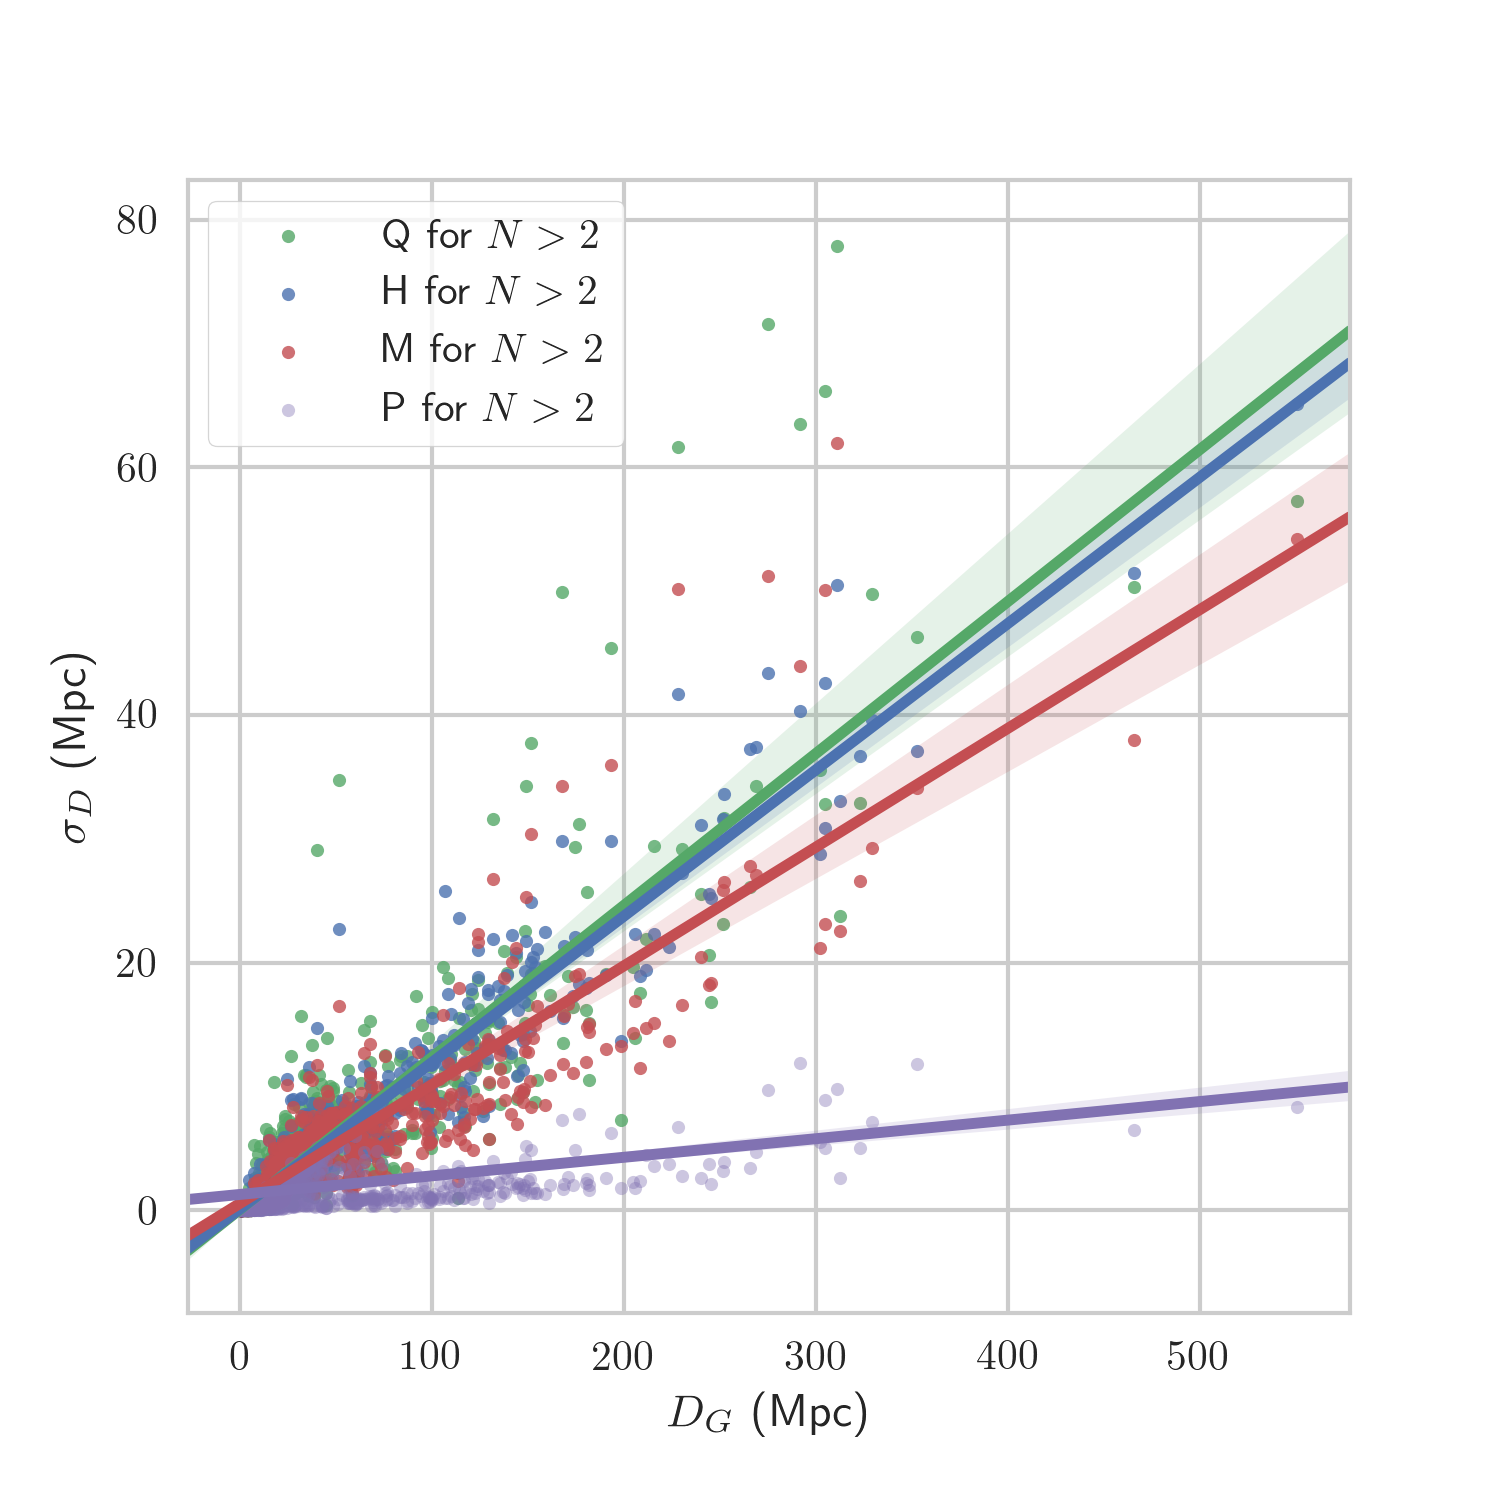
\includegraphics[scale=0.7]{HLhigh.png}
    \caption{Median extragalactic distance vs. predicted extragalactic distance errors for galaxies with more than 2 redshift-independent distance measurements in HyperLEDA according to the H, M, Q, P error models, showing a linear regression and confidence intervals computed using the \texttt{seaborn.regplot} Python function.}
    \label{fig:HLhigh}
\end{figure*}
HyperLEDA has 2473 distance measurements without reported errors for 1073 galaxies, of which 225 galaxies do not have any errors reported. Of these, 152 have FP and 34 have TF measurements. As mentioned in Section~\ref{sec:pred}, due to the low number of galaxies with more than 10 FP distance measurements we will not attempt to make a prediction of those missing errors. However, we can create synthetic errors for the 71 galaxies for which their only TF distance measurements have no-reported-error (incuding the 34 mentioned above) using our Bayesian predictive models for H and M TF errors. Predicted H errors are somewhat higher than those estimated for HyperLEDA, although acceptably within the range (Fig.~\ref{fig:predhl1}). On the other hand, predicted M errors are very close to the HyperLEDA M error estimates (Fig.~\ref{fig:predhl2}). This is remarkable, considering that here we are not filtering by method, as we did in Figs.~\ref{fig:predl1} and Figs.~\ref{fig:predl2} above.
\begin{figure*}
	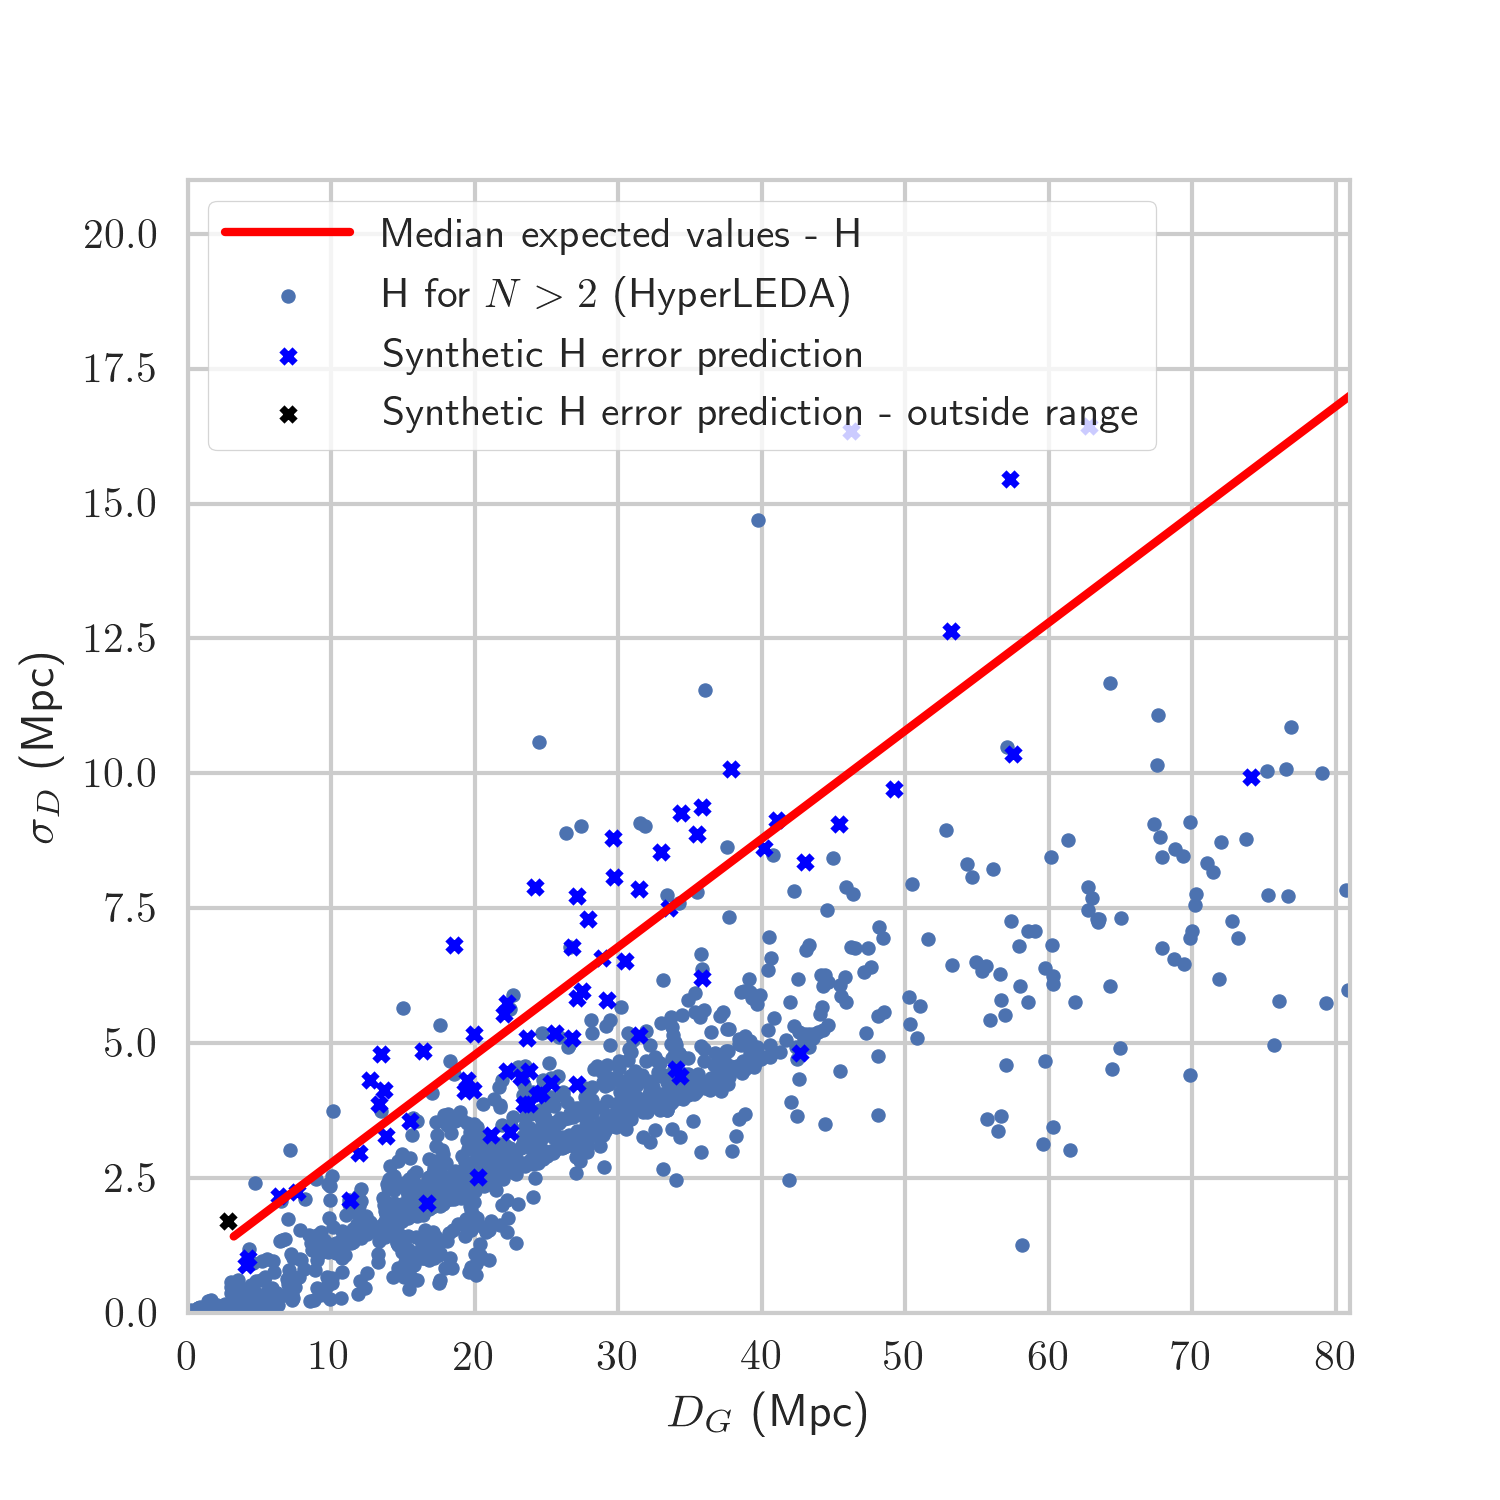
\includegraphics[scale=0.7]{predhl1.png}
    \caption{Synthetic H-method $\sigma_D$ and their median expected values for the 71 galaxies in HyperLEDA for which no TF distance measurements report an error, generated using the corresponding Bayesian linear model. Predicted errors for galaxies outside of the working distance range of the model are plotted in black. H errors for galaxies with more than 2 distance measurements are also plotted for comparison.}
    \label{fig:predhl1}
\end{figure*}
\begin{figure*}
	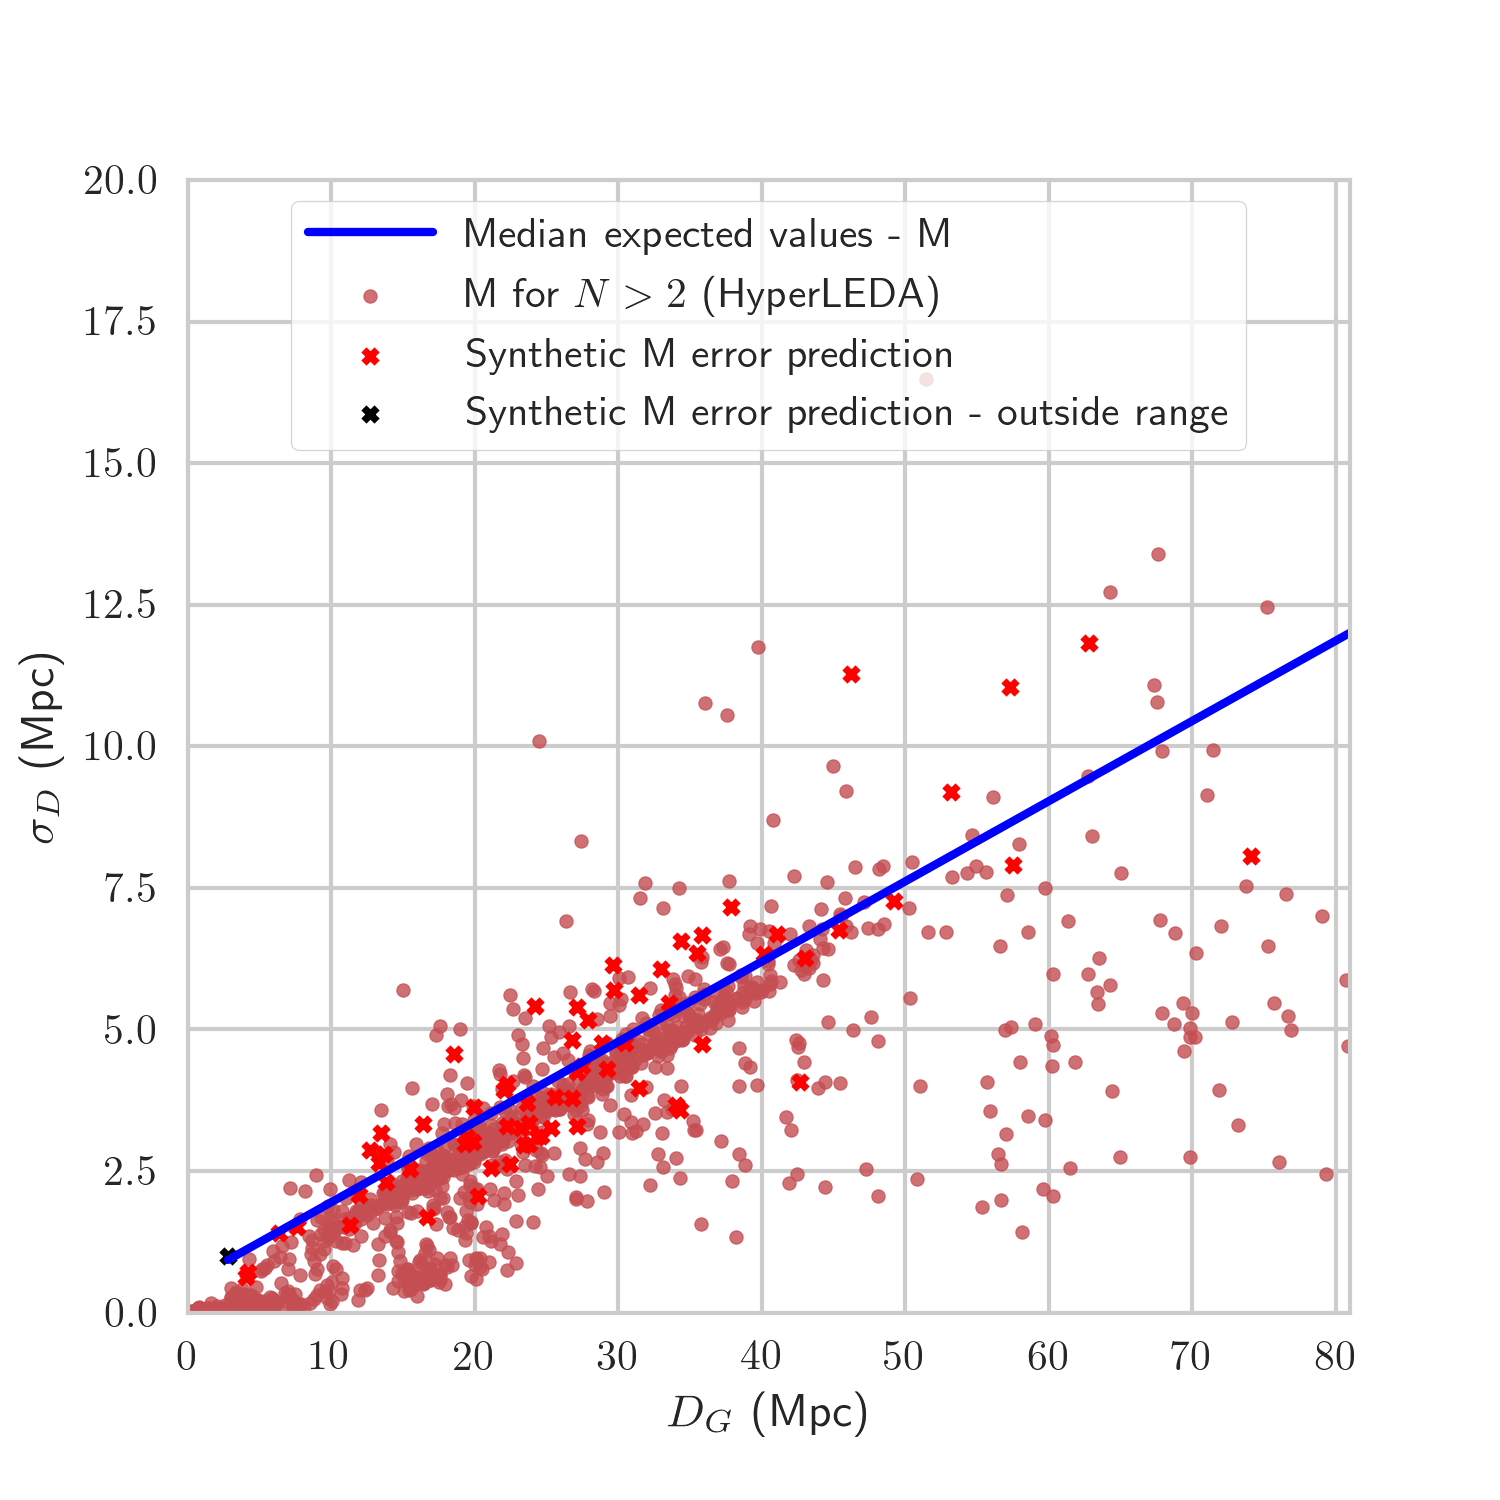
\includegraphics[scale=0.7]{predhl2.png}
    \caption{Synthetic M-method $\sigma_D$ and their median expected values for the 71 galaxies in HyperLEDA for which no TF distance measurements report an error, generated using the corresponding Bayesian linear model. Predicted errors for galaxies outside of the working distance range of the model are plotted in black. M errors for galaxies with more than 2 distance measurements are also plotted for comparison.}
    \label{fig:predhl2}
\end{figure*}
Bootstrap H and M treatment for HyperLEDA, NED-D and Cosmicflows-3, along with plots (3 plots total) and tables. 
%Don't forget  abstract. Change repo location (better name).
%NED-D per-method error - neglect missing errors for galaxies that have other TF measurements with reported error.
%generative per-method HQMP plots for NED-D? put them all in one page - overkill?
%cite number of methods per catalog?
%%%%%%%%%%%%%%%%%%%%%%%%%%%%%%%%%%%%%%%%%%%%%%%%%%

%\citep[e.g.][]{photred1}.
%Figures are referred to as e.g. Fig.~\ref{fig:example_figure}, and tables as
%e.g. Table~\ref{tab:example_table}.
% Example table
%\begin{table}
%	\centering
%	\caption{This is an example table. Captions appear above each table.
%	Remember to define the quantities, symbols and units used.}
%	\label{tab:example_table}
%	\begin{tabular}{lccr} % four columns, alignment for each
%		\hline
%		A & B & C & D\\
%		\hline
%		1 & 2 & 3 & 4\\
%		2 & 4 & 6 & 8\\
%		3 & 5 & 7 & 9\\
%		\hline
%	\end{tabular}
%\end{table}



% Don't change these lines
\bsp	% typesetting comment
\label{lastpage}
\end{document}

% End of mnras_template.tex